\documentclass[usenatbib,fleqn]{mnras}

\makeatletter
\newlength{\abovecaptionskip}%
\setlength{\abovecaptionskip}{10\p@}
\makeatother


\usepackage{threeparttable}
 

\usepackage{amsmath,amssymb}
\usepackage{mathrsfs}
\usepackage{graphicx}
\usepackage{epstopdf}
%\usepackage{hyperref}
\epstopdfsetup{outdir=./figures/}
\graphicspath{{./figures/}}
\usepackage{url}
%\usepackage{aas_macros}

\newcommand\lsim{\mathrel{\rlap{\lower4pt\hbox{\hskip1pt$\sim$}}
    \raise1pt\hbox{$<$}}}
\newcommand\gsim{\mathrel{\rlap{\lower4pt\hbox{\hskip1pt$\sim$}}
    \raise1pt\hbox{$>$}}}


\newcommand       \be          {\begin{eqnarray}}
\newcommand       \ee          {\end{eqnarray}}
\newcommand{\Mbh}[1][]{M_{\bullet#1}}
\newcommand{\Menc}{M_{\rm enc}}
\renewcommand{\th}{t_h}
\newcommand{\Msun}{{\rm M_\odot}}
\newcommand{\pyear}{{\rm yr}^{-1}}
\newcommand{\rs}{r_s}

% write title (with email and institute)
\title{The influence of environment on radio emission from TDE jets}
\author[Generozov et al.]{ A. Generozov$^{1}$, P. Mimica$^{2}$,
  B. D. Metzger$^{1}$,
  D. Giannios$^{3}$, 
  N. Stone$^{1}$,
  M.A. Aloy$^{2}$ 
  \\
  $^{1}$Columbia Astrophysics Laboratory, Columbia University, 550 West 120th Street, New York, NY 10027\\
  $^{2}$Departamento de Astronomia y Astrofisica, Universidad de Valencia, E-46100 Burjassot, Spain\\
  $^{3}$Department of Physics and Astronomy, Purdue University, 525
  Northwestern Avenue, West Lafayette, IN 47907, USA}

\begin{document}
\maketitle
\begin{abstract}
  There are now dozens of candidates for tidal disruptions of stars by
  supermassive black holes (TDEs) in optical and x-rays. A small
  fraction of these events, (e.g. Sw-J1644+57) have radio emission
  consistent with a powerful, relativistic jet interacting with
  surrounding nuclear gas. A priori it is not clear if the small
  number of observed relativistic TDEs is due to an intrinsic lack of jets
  or unfavorable nuclear gas densities for producing observable radio
  emission. We test the second possibility by calculating radio
  light curves for jets interacting with a broad range of density
  profiles, bracketing the expected range of gas densities in galactic
  nuclei ($\sim$ 0.5-1000 cm$^{-3}$ at $10^{18}$ cm). We find bright radio
  transients across the entire range of expected density
  profiles. Existing radio upper limits are often taken decades after
  the observed flare, well after the expected peak of the light curve
  for low density environments. Nonetheless they exclude powerful,
  Sw-J1644-like jets for CNM densities less than 60 cm$^{-3}$ at
  $10^{18}$ cm. More stringent constraints would be possible with
  prompt follow-up of tidal disruption event candidates and would
  inform our understanding jet launching physics.
\end{abstract}
\section{Introduction}
\label{sec:intro}
When a star in a galactic nucleus is deflected too close to the
central supermassive black hole (BH), it can be torn apart by tidal
forces.  During this tidal disruption event (TDE), roughly half of the
stellar debris remains bound to the BH, while the other half is flung
outwards and unbound from the system.  The bound material, following a
potentially complex process of debris circularization
(\citealt{Guillochon+2013},\citealt{Hayasaki+2013},\citealt{Hayasaki+2015},\citealt{Shiokawa+2015},\citealt{Bonnerot+2015}),
accretes onto the BH, creating a luminous flare lasting months to
years \citep{Hills1975, Carter+1982, Rees1988}.

Many thermal TDE flares have now been identified at UV/optical
\citep{van-Velzen+2011, Gezari+2012, Chornock+2014, Arcavi+2014} and
soft x-ray wavelengths \citep{Esquej+2007}.  Beginning with the
discovery of {\it Swift} J1644+57 in 2011, three additional TDEs have
been discovered by their non-thermal x-ray emission
(\citealt{Bloom+2011, Levan+2011, Burrows+2011, Zauderer+2011,
  Cenko+2012, Pasham+2015, Brown+2015}).  Unlike the thermal TDEs,
these events are the result of emission from a transient relativistic
jet beamed along our line of sight, similar to the blazar geometry of
active galactic nuclei (AGN).  In addition to their highly variable
X-ray emission, which likely originates from the base of the jet,
these events are characterized by radio synchrotron emission.  The
latter, more slowly evolving, is powered by shocks formed at the
interface between the jet and surrounding circumnuclear medium (CNM)
(\citealt{Giannios&Metzger2011,Metzger+2012}), analagous to the
afterglow of a gamma-ray burst.

Although a handful of jetted TDE flares have been observed, their
volumetric rate is a very small fraction $\sim 10^{-5}-10^{-4}$ of the
rate of the observed thermal TDE flares (e.g., \citealt{Burrows+2011},
\citealt{Brown+2015}), and an even smaller fraction of the
theoretically predicted TDE rate (\citealt{Stone&Metzger2016}).  One
potential explanation for this discrepancy is that the majority of
TDEs produce powerful jets, but their non-thermal X-ray emission is
relativistically beamed into a small angle $\theta_{\rm b}$, making
them visible to only a small fraction of observers.  However, the
inferred beaming fraction $f_b \approx \theta_{b}^{2}/2 \sim
10^{-5}-10^{-4}$ would require $\theta_{\rm b} \sim 0.01$ and hence a
jet with a bulk Lorentz factor of $\Gamma \gtrsim 1/\theta_j \sim
100$, much higher than typically inferred for AGN jets or inferred for
{\it Swift} J1644+57 (\citealt{Metzger+2012}) {\bf AG estimate of
  jetted fraction. Jetted event rate went down with other events due
  to larger co-moving volume, but there is considerable uncertainty in
  the TDE rate and hence the presented range.}.

The low detection rate of non-thermal TDE may instead indicate that
jets are intrinsically rare in TDEs, or the conditions of the
surrounding environment are unfavorable for producing bright emission.
Jets could be rare if they require, for instance, a highly
super-Eddington accretion rate (\citealt{De-Colle+2012}), a TDE from a
deeply plunging stellar orbit (\citealt{Metzger&Stone2015}), or a
particularly strong magnetic flux threading the star
(\citealt{Tchekhovskoy+2014,Kelley+2014}).  Alternatively, jet formation
or its X-ray emission could be suppressed if the disk undergoes
Lens-Thirring precession due to a misalignment between the angular
momentum of the BH and that of the disrupted star
(\citealt{Stone&Loeb2012}).  In the latter case, however, even a `messy'
jet could still be produced, which emits luminous non-thermal radio
synchrotron emission as it interacts the surrounding CNM.  The radio
emission from an off-axis is predicted to be relatively isotropic
(\citealt{Giannios&Metzger2011},\citealt{Mimica+2015}).

Observational campaigns have been conducted to follow-up thermal TDE
flares at radio wavelengths on timescales of months to decades after
the outburst (\citealt{Bower+2013}; \citealt{van-Velzen+2013}; see
Table 1 of \citet{Mimica+2015} for a compilation). Neither of these
campaigns found any radio afterglows definitively associated with the
host galaxies of strong thermal TDE candidates.\footnote{There were
  radio detections for two ROSAT flares: RX J1420.4+5334 and IC
  3599. However, for RX J1420.4+5334 the radio emission was observed
  in a different galaxy than was originally associated with the flare.
  IC 3599 has shown multiple outbursts in the calling into question
  whether it is a true TDE at all \citep{Campana+2015}.}
\citet{Bower+2013} and \citet{van-Velzen+2013} use a simple model for
the radio emission as a Sedov blast wave, to conclude that $\lesssim
10\%$ of TDEs produce jetted TDE emission at a level similar to that
produced in {\it Swift} J1644+57.  \citet{Mimica+2015} used 2D
hydrodynamical models, coupled with a synchrotron radiation transport
calculation, to model the on-axis emission from {\it Swift} J1644+57,
which they then extended to the case of an off-axis viewing angle to
conclude that most previous TDEs should have been detected if their
jets were as powerful.

Previous works (\citet{Bower+2013}; \citet{van-Velzen+2013};
\citealt{Mimica+2015}) have generally assumed that all TDEs occur in a
similar environment as {\it Swift} J1644+57.  However, in general the
gas density in a galactic nucleus depends sensitively on the sources
of gas from stellar winds, and the sources of gas heating
(\citealt{Quataert2004,Generozov+2015}).  In a gamma-ray
burst, the environment the jet emerges is relatively well-understood
to be the wind of the massive progenitor star, or the ISM of the host
galaxy.  However, in a TDE, the density could in principle be orders
of magnitude higher.

In this paper we address the range of gas densities encountered by
jetted TDEs and estimate their synchrotron emission by means of
analytic calculations and numerical simulations.  If we find radio
emission should be detected for all plausible CNM densities, then we
are lead to the conclusion that most TDEs do not launch J1644-like
jets.  This result would have significant implications for the physics
of jet launching in TDEs and more broadly.

In $\S\ref{sec:cnm}$ we explore the expected CNM densities using the
formalism developed in \citet{Generozov+2015} (hereafter GSM15) to
calculate the CNM profile for different assumptions about the stellar
population in the galactic nucleus.  A younger stellar population
produces significant wind mass loss from O \& B stars. In contrast,
the rate of wind mass loss from an older population, which lacks these
massive stars, could be $\sim 2$ orders of magnitude smaller.  We show
that the requirement of a physical stellar population limits the gas
density on a scale of $10^{18}$ cm to a range of $n_{18} \sim
1-10^{3}$ cm$^{-3}$. We also show that the measured distribution
of Eddington ratios suggests that the gas density in most galaxies is
bracketed by this range.

As a second component of this paper, in $\S\ref{sec:jet}$ we
explore the expected synchrotron emission from J1644+57-like across
the allowed range of CNM conditions.  We start in
$\S\ref{sec:analytic}$ with analytic conditions.  Then in
$\S\ref{sec:numerical}$ use both 1D and 2D hydrodynamic models to
simulate the jet propagating through the CNM and compare the results
in $\S\ref{sec:2D}$. In $\S\ref{sec:results}$ we show radio
light curves from our 1D models for a wide range of CNM densities, to
illustrate qualitatively how much varying the CNM density by itself
could change the radio light curve.  We summarize our conclusions in
$\S\ref{sec:conc}$.

\section{Range of CNM Densities}
\label{sec:cnm}

In this section we place theoretical and observational constraints on
the radial profile of the gas density $n(r)$ in the nuclei of
galaxies. 

\subsection{Analytic Constraints on CNM Density}

\subsubsection{Dynamical Model}
\label{sec:model}

The dominant source of gas injection into the CNM of quiescent
galaxies is winds from stars in the galactic nucleus. We model this
using the 1D spherical hydrodynamic equations with stellar wind mass
injection (e.g. \citealt{Holzer+1970}; \citealt{Quataert2004})
\begin{align}
  &\frac{\partial \rho}{\partial t}+\frac{1}{r^2}\frac{\partial}{\partial r}\left(\rho r^2 v\right)=q \label{eq:drhodt}\\
  &\rho \left(\frac{\partial v}{\partial t} + v\frac{\partial
      v}{\partial r}\right) =-\frac{\partial p}{\partial r}- \rho\frac{GM_{\rm enc}}{r^{2}} -q v \label{eq:dvdt}\\
  &\rho T\left(\frac{\partial s}{\partial t} + v\frac{\partial
      s}{\partial
      r}\right)=q\left[\frac{v^2}{2}+\frac{v_w^2}{2}-\frac{\gamma}{\gamma-1}
    \frac{p}{\rho} \right] ,
\label{eq:model}
\end{align}
where $\rho = \mu m_p n$, $v$, $p$, and $s$ are the density, velocity,
pressure (assumed to be an ideal gas with $\mu = 0.62$), and specific
entropy, respectively.  The enclosed mass $\Menc = M_{\bullet} +
M_{\star}$ includes both the black hole mass $M_{\bullet}$ and
enclosed stellar mass $M_{\star} \propto \int \rho_{\star}r^{2}dr$. 

The mass source term $q =\eta \rho_\star/\th$ is the mass injection
rate per unit volume per unit time, where $\rho_\star$ is the stellar
density. The energy source term $\propto v_w^{2}$, parameterizes the
heating rate of the gas, as physically results from stellar wind
kinetic energy, supernovae, and black hole feedback.

As described in \citet{Generozov+2015}, we have analytic approximations
for the densities and temperatures of steady state solutions to
equation~\eqref{eq:model}. We will apply these analytic formulas
across the physical range heating rates ($v_w$) and mass injection
rates ($\eta$), to obtain the physical range of CNM gas densities.

\subsubsection{Stellar density profiles}
We assume a broken power law for the stellar density profile, $\rho_{\star}$.
This is motivated by \citet{Lauer+2007} who use {\it
  Hubble Space Telescope} WFPC2 imaging to measure the radial surface
brightness profiles for hundreds of nearby early type galaxies. The
measured profile is well fit by a ``Nuker'' law parameterization:
i.e., a broken power law that smoothly transitions from an inner power law
slope, $\Gamma$, to an outer power law slope, $\beta$, at a break
radius, $r_b$.

Most galaxies have $0<\Gamma<1$, and are classified into two broad
categories: cores with $\Gamma<0.3$ and cusps with
$\Gamma>0.5$. Assuming spherical symmetry and a constant mass-to-light
ratio, the inner stellar profile translates to a stellar density
$\rho_\star\propto r^{-1-\Gamma}=r^{-\delta}$. Core galaxies have
$1<\delta<1.3$, while cusps have $1.5<\delta<2$.

Cusps are more common than cores for low mass black holes ($\Mbh\lsim
10^{8} \Msun$) relevant to TDEs. Additionally, as described in
\citet{Stone&Metzger2016} TDEs preferentially occur cuspy
galaxies. Using the tabulated TDE rates in Table C of
\citet{Stone&Metzger2016} we find a rate weighted average Nuker
$\Gamma$ of $\sim 0.7$. We adopt this $\Gamma$ (and the corresponding
stellar density power law slope $\delta=1.7$), as fiducial.

 {\bf Recently changed from $\delta=1.8$, need to
  double check all expressions.}

\subsubsection{Gas density profiles}
The radio emission produced by a TDE jet is most sensitive to the gas
density at the ``Sedov'' or deceleration radius, where the jet has
swept up it's own mass in nuclear gas. For Swift 1644 the deceleration
radius of the jet was $\sim 10^{18}$
cm \citep{Mimica+2015}. Thus, we focus on determining the nuclear gas
density as $10^{18}$ cm, $n_{18}$.  

In the presence of strong heating, one-dimensional steady-state flow
is characterized by an inflow-outflow structure, with a critical
radius known as the ``stagnation radius'', $\rs$, where the radial
velocity passes through zero.  Mass loss from stars interior to the
stagnation radius is accreted, while that outside $\rs$ is unbound in
an outflow from the nucleus.  It is most convenient to
first calculate $n(\rs)$ and then infer $n_{18}$. 

Fig.~\ref{fig:profiles} shows steady state gas density profiles
calculated for a core and a cusp stellar density profile. We mark the
stagnation radius, $r_s$, as a blue dot on each profile. As described
in \citet{Generozov+2015}, $r_s$ can be calculated analytically from the
heating rate ($v_w$) and black hole mass ($M$):

\begin{equation}
r_s \approx f(\delta) \frac{G M}{v_w^2},
\label{eq:rs}
\end{equation}


where $f(\delta)$ is an order unity function of the stellar density slope.
The density at the stagnation radius, $n(\rs)$ is determined by
injection rate of stellar wind material inside of $\rs$,
$\dot{M}$. This is proportional to the stellar mass enclosed inside of
$\rs$, $M_{\star}(\rs)$:

\begin{equation}
\dot{M}=\frac{\eta M_{\rm \star}(\rs)}{t_h}
\label{eq:dotM}
\end{equation}

At the sphere of influence, $r_{\rm inf}$, $M_{\star}(r_{\rm
  inf})=\Mbh.$ We take $r_{\rm inf}=3.5 \Mbh[,7]^{0.6}$, where
$\Mbh[,7]=\Mbh/10^7 \Msun$. Then for our
fiducial $\delta=1.7$,

\begin{equation}
\dot{M}= 3.0 \times 10^{-6} \Mbh[,7]^{0.22} \eta_{0.02} \left(\frac{r_s}{\rm
  pc}\right)^{1.3} \Msun \, {\rm yr}^{-1},
\end{equation}


where $\eta_{0.02}=\eta/0.02$. The density at the stagnation radius,
$n(\rs)$, can be estimated by equating the gas injected by stellar
winds over a free-fall time at the stagnation radius, $t_{\rm ff}
(\rs)$, to the gas mass enclosed inside of the stagnation radius:

\begin{align}
  &\frac{4 \pi}{3} \rs^3 \mu m_p n(r_s) \approx \dot{M} t_{\rm ff}
  (\rs) \nonumber\\
  &n(r_s) = 0.21 \eta_{0.02} \Mbh[,7]^{-0.28} \left(\frac{r_s}{\rm
      pc}\right)^{-0.2}
\label{eq:nrs}
\end{align}
 
Using equation~\eqref{eq:rs}, for $r_s$, we obtain 

\begin{equation}
n(r_s)=0.3 \, v_{500}^{0.6} \eta_{0.02} \Mbh[,7]^{-0.52} {\rm cm}^{-3},
\label{eq:nrs2}
\end{equation}

where $v_{500}=v_w/\left(500 \,\mathrm{km/s}\right)$. In the vicinity of
the stagnation radius, we find that the slope of the gas density
profile is $\sim (4\delta-1)/6$. For our fiducial $\delta$, 1.7, this
gives $n(r)\propto r^{-1}$ near $\rs$. Furthermore, the density
profile remains close to $n\propto r^{-1}$ for small radii of
interest.\footnote{For cusp galaxies, the gas velocity asymptotes to a
  constant between the stagnation radius and break radius (if they are
  sufficiently far apart). In this region we expect $n\propto
  r^{1-\delta}$.}  Thus, we adopt $n(r)= n_{18} (r/10^{18} {\rm
  cm})^{-1}$ as our fiducial density profile.  We also experiment with
a core-like density profile (appendix~\ref{app:core}), and compare the
radio light curves for jets going through core and cusp-like density
profiles in $\S\ref{sec:profileComp}$.


From our fiducial $n\propto r^{-1}$ and equation~\eqref{eq:nrs2}, we
obtain

\begin{equation}
n_{18}\simeq 0.3 \Mbh[,7]^{0.49} \eta_{0.02} v_{500}^{-1.5} {\rm
  cm^{-3}}.
\label{eq:n18}
\end{equation} 


In general the gas density steepens at the stellar break radius, $r_b$
(see Fig.~\ref{fig:profiles}). However, such breaks will only be
important if $r_b$ is inside of the Sedov radius, where the jet
sweeps up its own mass in CNM gas.  The jet mostly decelerates inside
of this radius, becoming Newtonian. Therefore, the profile outside of
this radius will be of minimal importance in shaping the radio
light curve. We plot the Sedov radius for different energy jets on
each of the profiles in Fig.~\ref{fig:profiles}. The measured break
radii of all but four the \citet{Lauer+2007} galaxies is larger than
10 pc. This is larger than the Sedov radius for even a very powerful
jet (isotropic equivalent energy $E=4\times 10^{54}$ erg), interacting
with a low density CNM ($n_{18}=2$). If a nuclear star cluster (NSC)
is present in the galactic center there will be a smaller effective
break radius at the outer edge of the NSC (typically 1-5 pc--see
\citealt{Georgiev+2014}). However, even for a break radius of 1 pc the
break radius will only be inside the Sedov radius for small densities
($n_{18}<20$) and powerful jets {\bf AG still feel that this is a
  relevant region of parameter space}. Henceforward we will not
consider the effects of the break radius in our analysis.


\begin{figure}
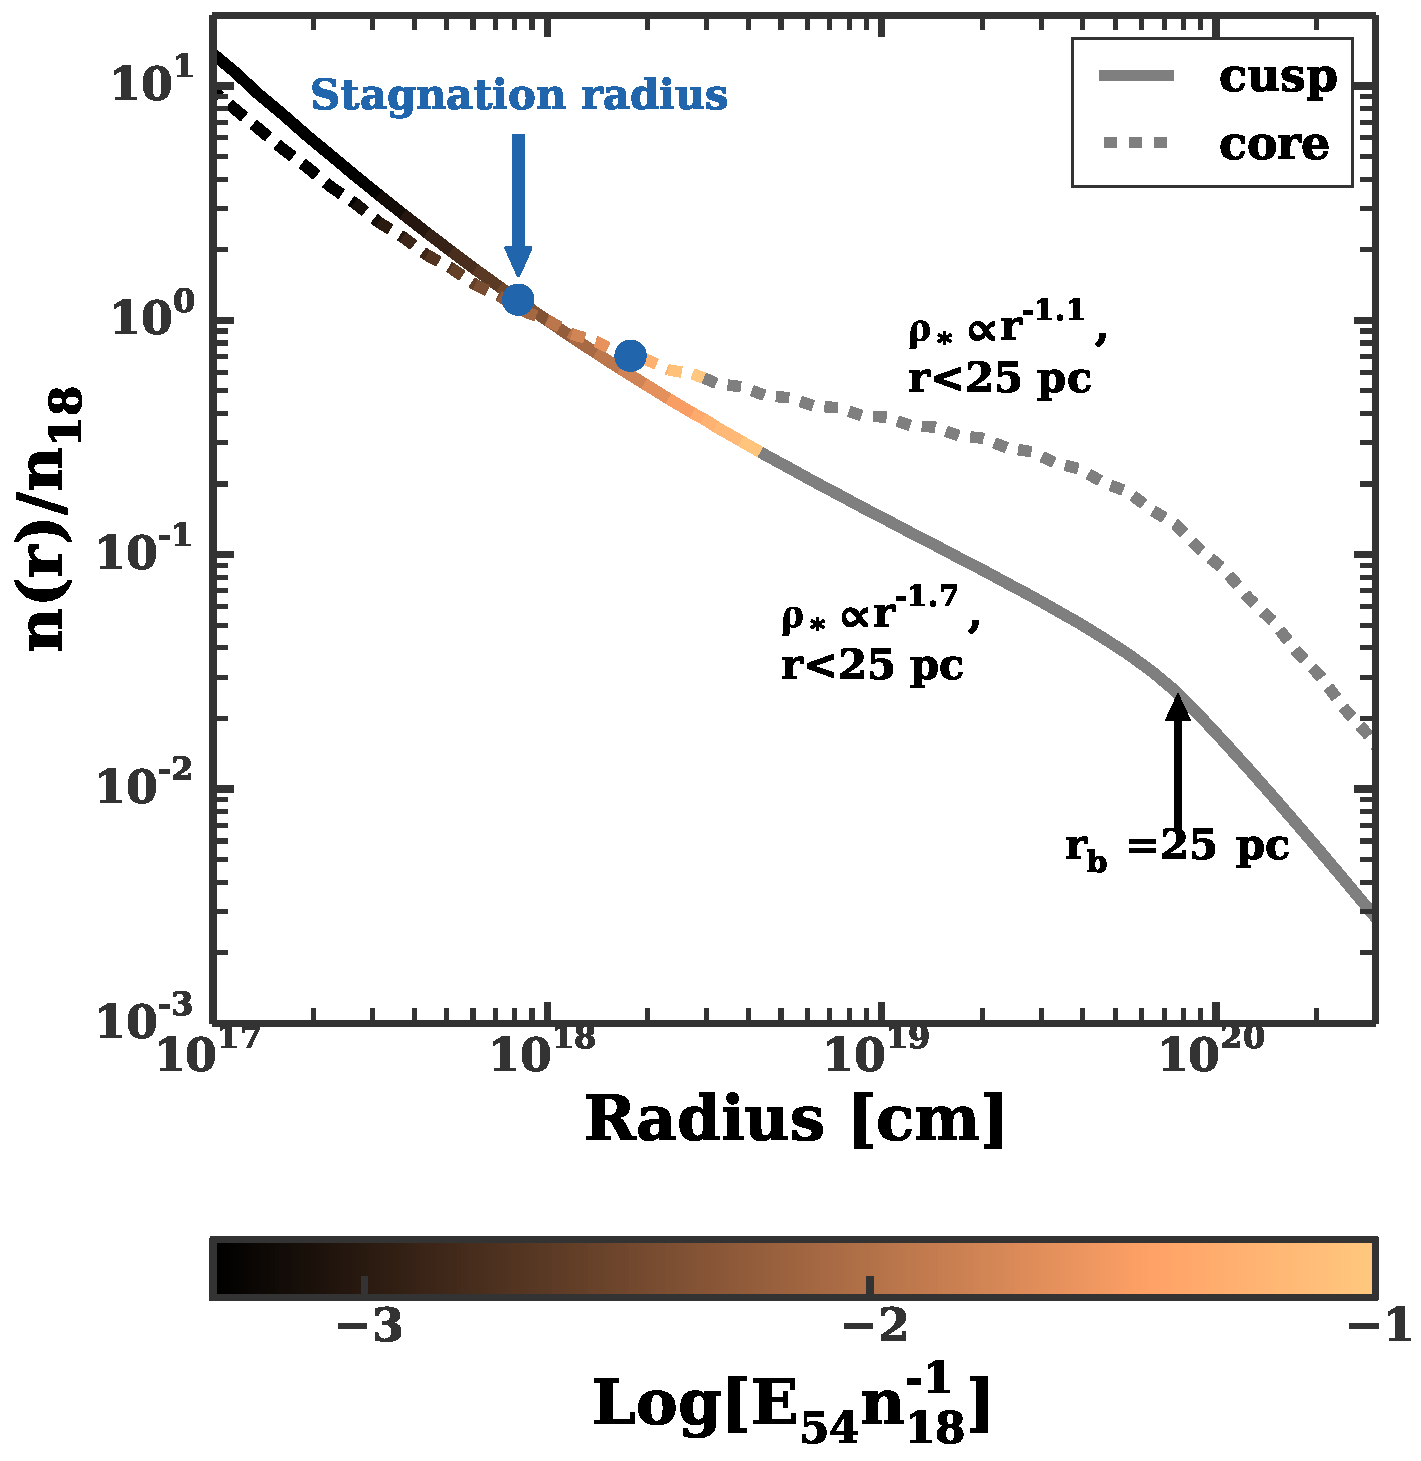
\includegraphics[width=8cm]{sedov_radius.pdf}
\caption{\label{fig:profiles} Steady state core and cusp density
  profiles. We have taken $\Mbh=10^{7} \Msun$ and $v_w$=600 km/s and
  both profiles have mass source function $q(r) \propto
  r^{-3}$ for $r > 25$. The core profile has $q(r) \propto
  r^{-1.1}$ for $r < 25$ and the cusp profile has $q(r)
  \propto r^{-1.8}$.  The colors at each radius indicate the value of
  isotropic jet energy $E_{52} n_{18}^{1}$, such that the gas mass
  inside that radius is equal to the mass inside the jet. We take the
  Lorentz factor of the un-shocked jet to be $\gamma_{\rm jet}=2$.
  Note that blue circles mark the location of the stagnation radius
      for each profile (where the gas velocity goes through 0).}
\end{figure}



\subsubsection{Plausible Density Range}
\label{sec:densAllowed}

We calculate the density at $10^{18}$ cm, $n_{18}$, for a range of
different star formation histories. 

We consider an old stellar population formed a Hubble time ago plus a
young component that formed a time $t_{\rm burst}$ ago and formed a
fraction $f_{\rm burst}$ of the stars. We assume that both the young
and old stars have the same (cuspy) density profile, which implies
that the gas density profile, $n\propto r^{-1}$. 

For a sufficiently large burst with $t_{\rm burst}<40$ Myr, heating
will be dominated by massive star winds.\footnote{Type II Supernovae
  are another important source of energy for young stellar
  populations. Overall the energy injected by O stars winds and Type
  II SNe will be comparable \citep{Voss+2009}. However, heating from
  Type II SNe will be intermittent and is not included here for
  simplicity.} In this case, we can calculate the mass return ($\eta$)
and heating parameters ($v_w$), using the procedure described in
GSM15. In this case $n_{18}$, can simply be calculated by using
equation~\eqref{eq:n18}.

For older stellar populations, heating may come from a few different
sources including Ia Supernovae or AGN feedback {\bf AG also unbound
  debris streams produced in tidal disruption events (see
  \citep{Guillochon+2015a})}. We focus on quiescent phases, where the
SNe Ia dominate. As discussed in GSM15 the Ias can clear the gas
inside of the Ia radius ($r_{\rm Ia}$), where the time between
successive Ia supernovae is equal to the dynamical time. To calculate
$n_{18}$, when Ias dominate the heating rate, we plug $r_{\rm Ia}$
into equation~\eqref{eq:nrs}, and extrapolate to $10^{18}$ cm. $r_{\rm
  Ia}$ is calculated as described in GSM15 for times $t>300 \,{\rm
  Myr}$. the Ia rate is given by $8.8 \times 10^{-13}
\left(\frac{t}{3\times 10^{8} {\rm yr}}\right)^{-1.12} \, \Msun^{-1} \,
{\rm yr}^{-1} $ for $t>3\times 10^8$ years. In GSM15 we incorrectly
extrapolated this rate all of the way to 3 Myr--this is clearly
un-physical as no white dwarfs would have formed by this time. Here,
we instead take the Ia rate to be 0 for times less than 40 Myr and
flat from 40 to 300 Myr.

Fig.~\ref{fig:param} shows how $n_{18}$ varies with star burst
properties ($f_{\rm burst}$ and $t_{\rm burst}$).  We find a maximum
$n_{18}$ of $\sim 2,700$ cm$^{-3}$, $\sim 4$ Myr after a burst of star
formation forming 100\% of the stars in the nucleus. In this case both
the energy an mass budgets are dominated by fast winds from massive
stars ($\gsim 15 \, \Msun$).  Although such a large gas density would
be present in the immediate aftermath of a starburst, the wind mass
loss rate (and hence the gas density) declines as $\eta \sim
t^{-3}$. This means, the gas density would decline by an order of
magnitude after just a few Myr.

The lowest density, $n_{18}\sim 0.03$ cm$^{-3}$ achieved for a
relatively modest burst, with $f_{\rm burst}=4\times 10^{-4}$. In this
case we have a high heating rate from the young, massive stars and a
low mass injection rate, with both young and old stars contributing.

In deriving this lower limit on the density, we assume that the
massive stars provide a spatially homogeneous heating source, even on
small scales. If this were true we would expect them to expel gas
outside of $r_s \sim 5\times 10^{16}$ cm. However, for the assumed
$f_{\rm burst}=4\times 10^{-4}$, we expect less than one massive star
inside of $r_s$.  In this case our formalism breaks down, and the true
density would be larger. For a simple estimate we set the location of
the stagnation radius by requiring it enclose one massive ($\gsim 15
\, \Msun$) star. This gives $r_s\sim 1.6\times 10^{18}$ cm. Plugging
this into equation~\eqref{eq:nrs} and taking $n\propto r^{-1}$ gives
$n_{18} \sim$ 0.5 cm$^{-3}$.

Discreteness effects will generically be important wherever, young
massive stars dominate the heating rate of the gas (hatched regions of
Fig.~\ref{fig:param}). 


A typical host galaxy for TDE has evidence of some star formation
within 1 Gyr \citep{French+2016}. This corresponds the right hand side
of Fig.~\ref{fig:param}. In this case the heating rate will be
dominated by Ia supernovae and $n_{18}\sim 80$ cm$^{-3}$.

{\bf Need to discuss thermal stability...}

 

\begin{figure} 
  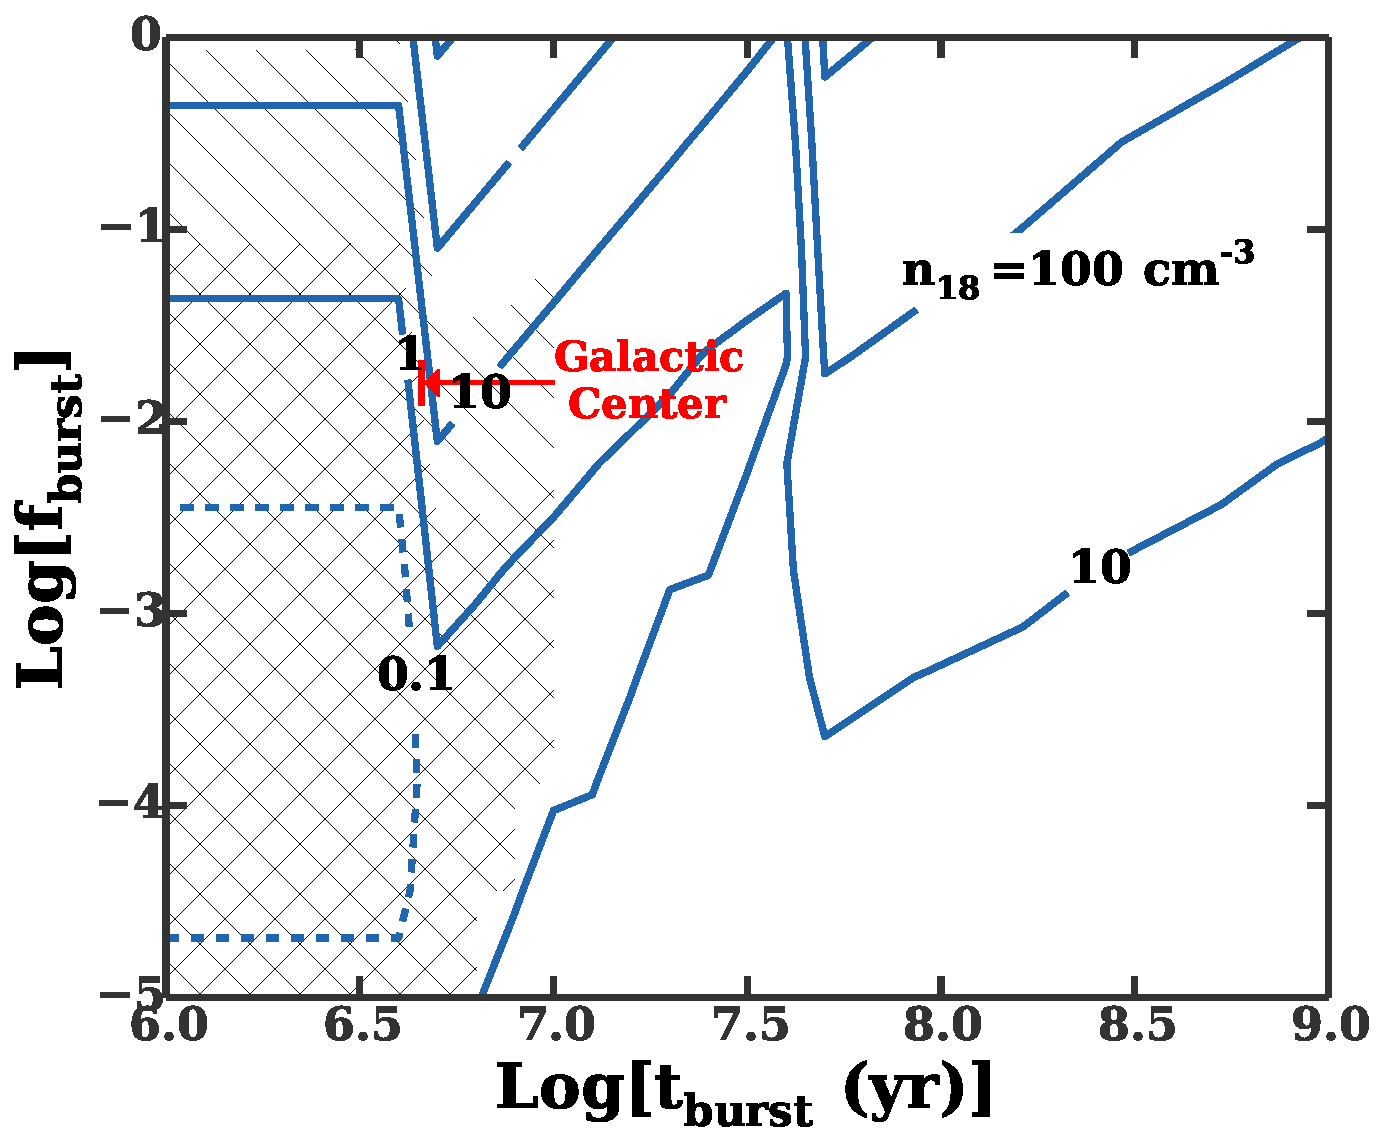
\includegraphics[width=8cm]{cnm_plot.pdf}
  \caption{\label{fig:param} Isocontours for the density at $10^{18}$
    cm ($\mathrm{n_{18}}$) (blue lines) for a $10^{7} \, \Msun$ black
    hole and bursts of star formation forming a fraction, $f_{\rm
      burst}$, of the stars $t_{\rm burst}$ years ago. We assume that
    the remaining stars had formed a Hubble time ago. We also 
    assume that the old and young stars have the same density
    profile. We mark regions of parameter space where approximations
    in our model would break down. Hatched areas indicate regions of
    parameter space, where massive stars ($\gsim 15 \, \Msun$)
    dominate the gas heating rate, but we would expect less than one
    (doubly hatched) or less than ten (singly hatched) massive stars
    inside the nominal stagnation radius (equation~\eqref{eq:rs}). In
    these regions of parameter space discreteness effects not captured
    by our formalism become important. In area inside of the red
    contours, the cooling time, $t_{\rm cool}$, becomes comparable to
    the free-fall time $t_{\rm ff}$, at the stagnation radius, with
    $t_{\rm cool}<10 t_{\rm ff}$ inside of the solid contour and
    $t_{\rm cool}< t_{\rm ff}$ inside of the solid contour. In this
    region radiative cooling and thermal instability become important
    (\textit{see text for discussion}).}
\end{figure}


\begin{figure}
  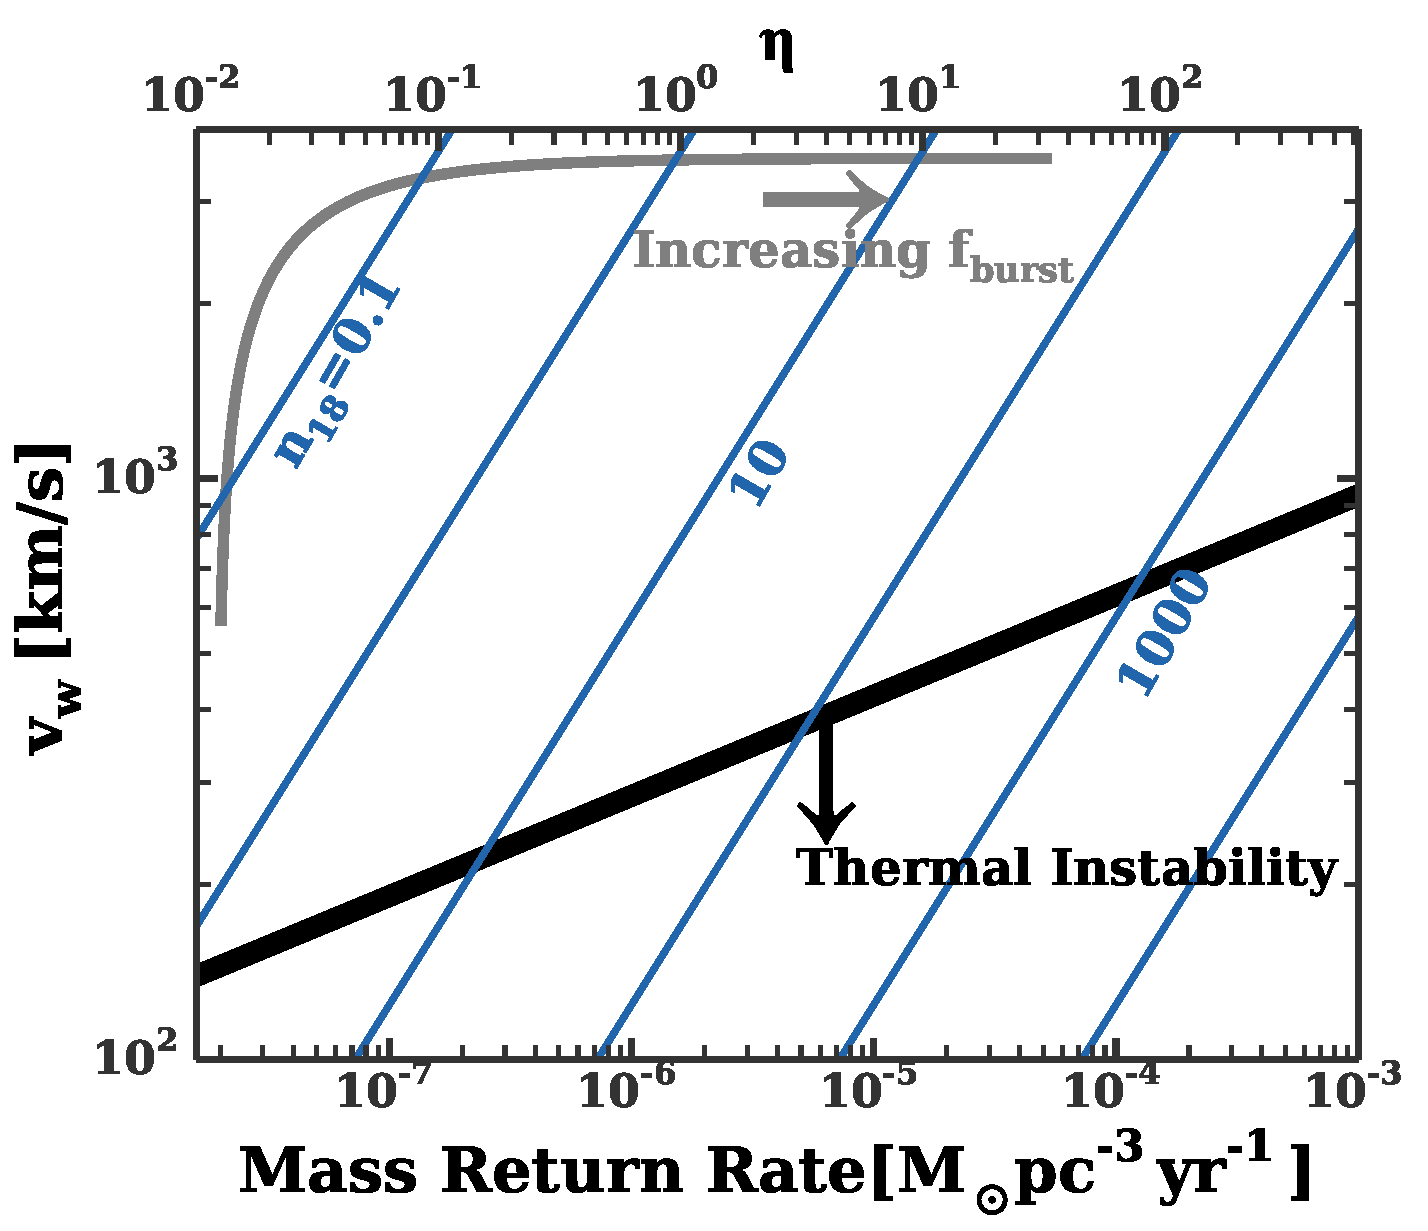
\includegraphics[width=8cm]{cnm_plot_2.pdf}
  \caption{\label{fig:param2} $n_{18}$ as a function of the mass
    return ($\eta$) and heating ($v_w$) parameters for a $10^7 \Msun$
    black hole. We translate the gray line from Fig.~\ref{fig:param}
    to this parameter space. $f_{\rm burst}$ increased in the direction
    indicated by the gray arrow. As indicated by the black solid line,
    the area below the black solid line is thermally unstable
    (\textit{see text for discussion}).}
\end{figure}

\subsection{Empirical Constraints on CNM Density}

In this section we translate observed constraints on the accretion
rate distribution of supermassive BHs into constraints on the CNM
density.  The density $n$ at radius $r$ can be written in terms of the
inflow rate, $\dot{M}$
\begin{equation}
\dot{M} = m \dot{M}_{\rm Edd}= f_{\rm in} 4 \pi r^2 \mu m_p n v,
\label{eq:mdot}
\end{equation}
where $n$ is the average density at radius $r$ and $f_{\rm in}$
represents the fraction of the large scale inflow, which actually
accretes onto the black hole.  If we assume that $r$ is interior to
the sonic radius, then we can approximate $v$ as the free-fall
velocity, $v_{\rm ff} = (2 G \Mbh/r)^{1/2}$.  In this case we
obtain
\begin{equation}
n_{18} = 3 \times 10^3 M_{\bullet,7}^{1/2} m f_{\rm in}^{-1} {\rm
  cm}^{-3}
\label{eq:n18Edd}
\end{equation}
We expect that $f_{\rm in}$ could be quite small for highly sub
Eddington systems. For example, Faraday rotation measurements
\citep{Quataert+2000} show $f_{\rm in}\approx 10^{-3}$, in our own
galactic center. However, we expect $f_{\rm in}$ will be of order
unity for systems with $m\gsim 0.1$.  

\citet{Kauffmann&Heckman2009} present distributions of the OIII line
luminosity, ${\rm L[OIII]}/\Mbh$, for a range of BH masses
($10^7-10^{8.5} \Msun$) from SDSS galaxies.  Assuming a bolometric
correction, these can be translated into distributions of Eddington
ratio $m$.  According to \citet{Kauffmann&Heckman2009} ${\rm
  L[0III]}/\Mbh=1.7$, roughly corresponds to Eddington ratio of 1. We
adopt this conversion and assume that the bolometric correction is
independent of ${\rm L[0III]}/\Mbh$. 

We can turn the distribution of $L/L_{\rm Edd}$ into a distribution of
$m=\dot{M}/\dot{M}_{\rm Edd}$, with a prescription for the radiative
efficiency $\epsilon_{\rm rad}$.  For $m \leq 0.01$, we refer to
\citet{Sharma+2007}, who estimate the radiative efficiency of low
luminosity AGN using MHD shearing box simulations.  They find (see
their Fig.~6)

\begin{align}
\epsilon_{\rm rad} \simeq 
\begin{cases}
  0.03 \left(\frac{\dot{M}_{\bullet}}{10^{-4}\dot{M}_{\rm edd}}\right)^{0.9} & \frac{\dot{M}_{\bullet}}{\dot{M}_{\rm edd}} \lsim 10^{-4} \\
 0.03 &  10^{-2} \gsim \frac{\dot{M}_{\bullet}}{\dot{M}_{\rm edd}} \gsim  10^{-4},
\end{cases}
\label{eq:efficiency}
\end{align}


with a large uncertainty (factor of 5 in either direction) for small
$m\lsim 10^{-4}$, as the radiative efficiency depends on uncertain
micro-physical parameters. We adopt equation~\eqref{eq:efficiency} for
$m <0.01$, $\epsilon_{\rm rad}=0.1$ for $m>0.1$, and linearly
interpolate between the two for intermediate values of $m$.

\begin{figure}
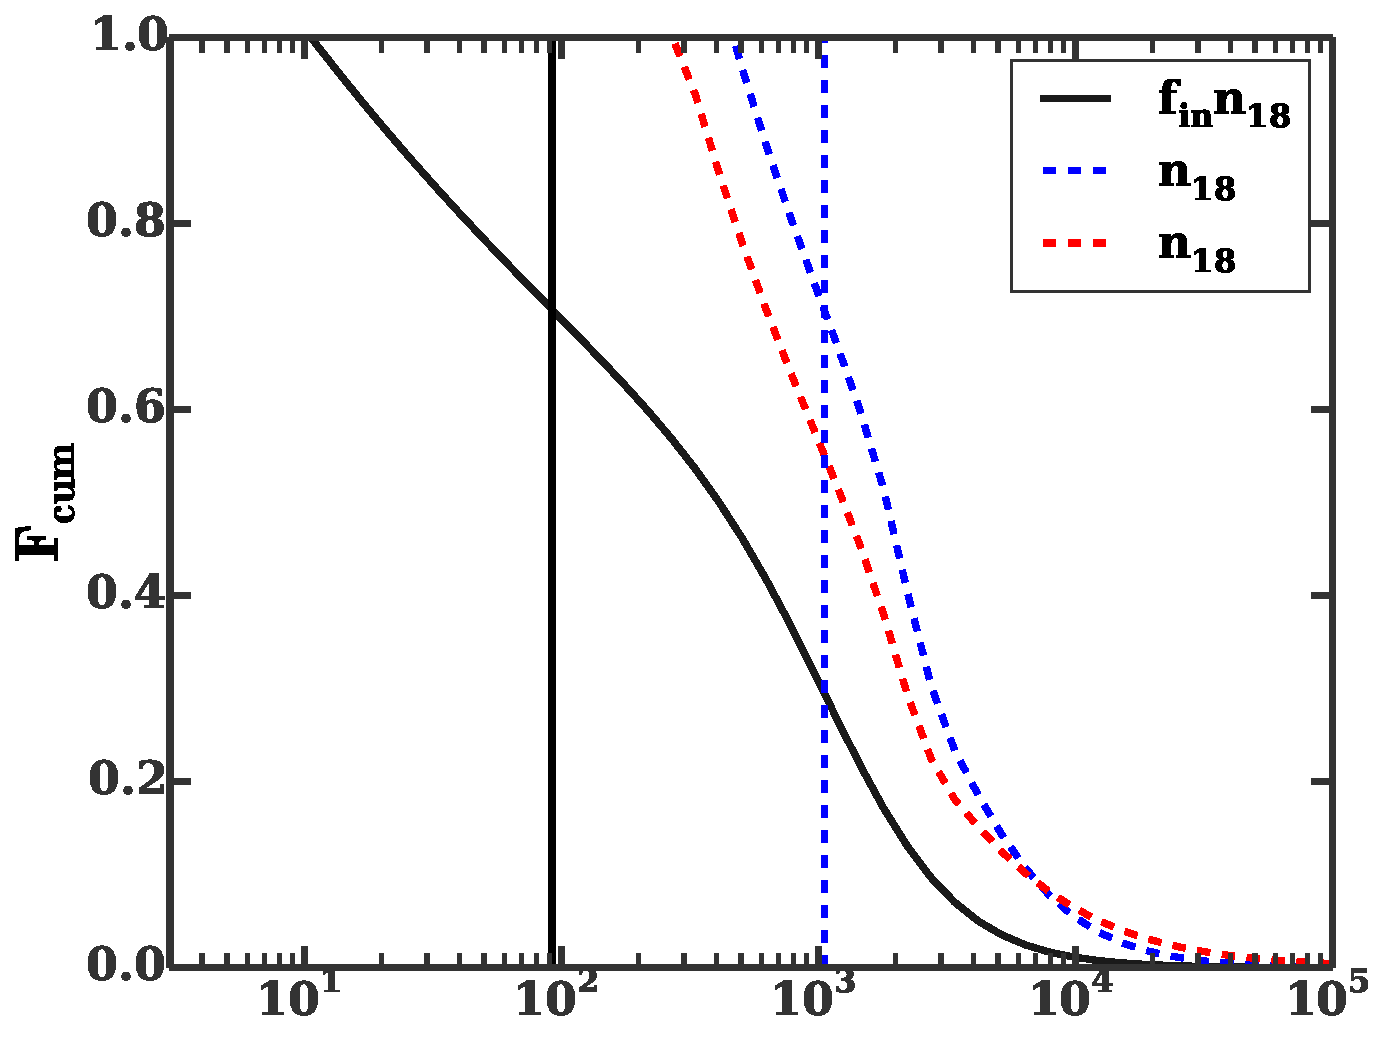
\includegraphics[width=8cm]{fcum_n18.pdf}
\caption{\label{fig:n18Cum} Cumulative distribution of $f_{\rm in}
  n_{18}$ for black holes with mass $\Mbh\simeq 10^{7} \Msun$ based on
  the observed cumulative distributions of Eddington ratios from
  \citet{Kauffmann&Heckman2009} {\it (solid black line)}. Recall that
  $f_{\rm in}$ is the ratio of the true accretion rate onto the black
  hole to the inflow rate of free-falling gas at $10^{18}$ cm.  The
  dashed blue line is the corresponding cumulative distribution of
  $n_{18}$, taking an $f_{\rm in}$ based on the simulations of
  \citet{Li+2013} ($\dot{M}_{\rm Acc}/\dot{M}_{\rm Bondi}$ in their
  Figure 6). The distribution of $f_{\rm in} n_{18}$ ($n_{18}$) is
  unreliable to the left of the solid black (dashed blue) vertical
  line. Such low densities correspond to systems with very small OIII
  luminosities, which could be coming from star formation rather than
  the black hole accretion flow.}
\end{figure}


Fig.~\ref{fig:n18Cum} shows the distribution of $n_{18}$ resulting
from combining this distribution with equation~\eqref{eq:n18Edd}.  The
absence of galaxies with $f_{\rm in }n_{18} \lsim$ few cm$^{-3}$
places a lower bound on $n_{18}$ of a few cm$^{-3}$.  However,
measurements of Eddington ratio below $\sim 10^{-3}$ (shown with a
vertical line in Fig.~\ref{fig:n18Cum}) are not reliable. This allows a
moderate fraction of galaxies ($\sim 30\%$) to have much lower gas
densities.


In order to obtain the cumulative distribution for $n_{18}$, we need a
prescription for $f_{\rm in}$. We refer to \citet{Li+2013}, who
performed two-dimensional hydro-dynamical simulations of axi-symmetric
rotating accretion flows. When the inflow rate on large scales was
very sub-Eddington ($\dot{M}/\dot{M}_{\rm Edd} \lsim 10^{-4}$),
cooling was inefficient and $f_{\rm in}$ was $\sim 0.01$. On the other
hand, when $\dot{M}/\dot{M}_{\rm Edd}\gsim 10^{-2}$, $f_{\rm in}$
approaches unity.  We use $\dot{M}_{\rm Acc}/\dot{M}_{\rm Bondi}$ in
their Figure 6 for $f_{\rm in}$.  With this choice only a third of
nuclei have $n_{18}>2,000$ and only 6\% have $n_{18}>10^{4}$. Note
that existing tidal disruption event candidates are unlikely to be in
the high density tail with either no sign or sign of or very weak AGN
emission lines (e.g. \citealt{van-Velzen+2011, Arcavi+2014}). 

Note that \citet{Li+2013} use an alpha viscosity prescription with
$\alpha=0.01$.  $f_{\rm in}$ would depend on this choice. This
uncertainty in $f_{\rm in}$ translates into a systematic uncertainty
in the distribution of $n_{18}$. 
 
Two potential complications to keep in mind are (i) clumpiness of the
CNM and (ii) anistropy. The distributions above are distributions of
the {\it average} $n_{18}$.  Most likely, some of the nuclear gas in a
low density hot phase, while the rest is in high density cold
clumps/filaments.  However, while the jet is relativistic the
light curve of a jet propagating through a clumpy medium will differ
little from that of a smooth medium with the same average
density. Even in the late stages when the jet becomes non-relativistic
clumps will only make a difference when the size of the clumps is
comparable to the size of the jets.

The cold gas could be distributed anistropically. For example it could
be could be concentrated in a ring-like structure. In this scenario,
the some fraction of jets would likely be stifled by the very dense
ring. However, such a ring would not block all jet propagation
directions. 

There may also be anisotropies present in the hot phase of gas. AGN
feedback would may blow low density bubbles in the
CNM. \citet{Russell+2013} used Chandra x-ray observations to measure
gas density and temperature profiles for a sample of massive
elliptical galaxies. The measured electron density on scales of $\sim
100$ pc is $\gsim 0.1$ cm$^{-3}$. Note that the gas density at 100 pc
would be irrelevant for a TDE jet, but we would not expect the gas
density to be decreasing towards the galactic center in a steady
state.  We note that massive black holes in the \citet{Russell+2013}
sample, with $\Mbh\sim 10^{9} \Msun$, whereas black holes tidal
disruption events would have $\Mbh\lsim 10^8 \Msun$. This is because
more massive black holes would not be able to disrupt (main sequence)
stars.


These empirical constraints nicely complement the analytic estimates
in the previous section. On the one hand, the distribution of
Eddington ratios becomes unreliable for low luminosities.  In this
case it is difficult to put a lower bound on the density
observationally. However, the analytics give a low density floor
expected from injection of stellar wind material ($\sim 0.5$
cm$^{-3}$). 

% On the other hand, the analytic estimates are specific to
% the hot phase of gas. The Eddington ratio distribution probes the
% average density (including any cold clumps). The
% distribution of Eddington ratios gives us confidence in our high
% density limit ($\sim 1000$ cm$^{-3}$).



\section{TDE jets}
\label{sec:jet}

\subsection{Analytic Considerations}
\label{sec:analytic}


The mass of CNM swept up by the jet $2\pi\theta_{\rm j}^{2}\int m_p
n_{\rm cnm}(r) r^{2}dr$ equals its own rest mass $M_{\rm j} = E_{\rm
  j}/\Gamma_{\rm j}c^{2} \approx \frac{E_{\rm iso}
  (\theta_j^2/2)}{\Gamma_j c^2} $ at the characteristic (`Sedov')
radius given by
n by

\begin{equation}
r_{\rm sedov} = E_{54}^{1/2} \Gamma_{10}^{-1/2} n_{\rm 18}^{-1/2}\,{\rm pc}, 
\end{equation}

where $E_{54}$ is the isotropic equivalent jet energy normalized to
$10^{54}$ ergs. We use our fiducial CNM density profile $n(r)=n_{18}
\left(r/10^{18} {\rm cm}\right)^{-1}$.

From the continuity equation, the (co-moving) density of the jet is
given by (e.g. Uhm \& Beloborodov 2007)
 \begin{align}
   n_{\rm j} =  \frac{L_{\rm j, iso}}{4 \pi r^{2}\Gamma_{\rm
       j}^{2}c^{3}m_p(1 + r \dot{\Gamma_{\rm j}}/c\Gamma_{\rm j}^{3})}
   \approx  \frac{L_{\rm j, iso}}{4 \pi r^{2}\Gamma_{\rm j}^{2}c^{3}m_p}
\end{align}

where the second term in the denominator is generally negligible as
long as the Lorentz factor of the jet changes slowly
$\dot{\Gamma}_{\rm j} \ll c\Gamma_{\rm j}^{3}/r$, as can be shown to
be true at radii $r < r_{\rm sedov}$ as long as $\Gamma_{\rm j}$
changes on timescales $\gtrsim t_{\rm j}$.

A critical parameter is the ratio of the density of the jet to the
CNM

\begin{equation}
  f\approx 40\,  L_{\rm j,48} n_{18}^{-1} \Gamma_{10}^{-2} \, \left(\frac{r}{10^{18} {\rm
        cm}}\right)^{-1} 
\end{equation}

For a given $f$, the Lorentz factor of the shocked material may be
calculated using the relativistic shock jump condition and pressure
equality between the forward and reverse shocks. In the
ultra-relativistic limit

\begin{equation}
\Gamma_{\rm sh} \underset{\Gamma_{\rm sh} \gg 1}= \Gamma_{\rm j}\left[1 + 2\Gamma_{\rm j}f^{-1/2}\right]^{-1/2}
\end{equation}

However, this expression is problematic when the outflow is mildly
relativistic or non-relativistic. In particular, it gives Lorentz
factors less than 1. A more general expression for $\Gamma_{\rm sh}$
can be obtained using equation 3 from
\citet{Beloborodov&Uhm2006}\footnote{As pointed out by
  \citet{Beloborodov&Uhm2006}, this expression may still be
  problematic as it assumes a constant pressure between the forward
  and reverse shocks.}

\begin{align}
&\frac{\Gamma_j^2-1}{\gamma_{43}^2-1} f^{-1}=1\\
&\gamma_{43}=\Gamma_j \Gamma_{\rm sh} \left(1-\beta_{\rm sh} \beta_j\right).
\label{eq:gammaShGen}
\end{align}

We use this expression to find the Lorentz factor when the reverse
shock crosses the bulk of the ejecta.  At a given snap-shot in time,
we have the Lorentz factor of the reverse shock (in the lab frame)

\begin{equation}
\Gamma_{\rm rs}=\frac{\beta_{\rm sh}(f)-\beta_{43}(f)/3}{1-\beta_{\rm
    sh}(f) \beta_{43}(f)/3}.
\end{equation} 

Then it is straightforward for a jet of a given thickness, $\delta$,
to find the radius where the reverse shock crosses the trailing edge
of the jet using equation~\eqref{eq:gammaShGen}.

We plot the fraction of the slow component ($\Gamma_j=2$) kinetic
energy dissipated by the reverse shock as a function of isotropic jet
luminosity and $n_{18}$ in Fig.~\ref{fig:diss}. For the purposes of
our analytic estimates, we assume a constant luminosity jet, which
shuts off after time $t_{\rm fb}=5 \times 10^{5}$ s. For the numerical
calculations described in the subsequent sections, the jet luminosity
declines as $t^{-5/3}$ after time $t_{\rm fb}$ (see equation~\ref{eq:lum}).


\begin{figure}
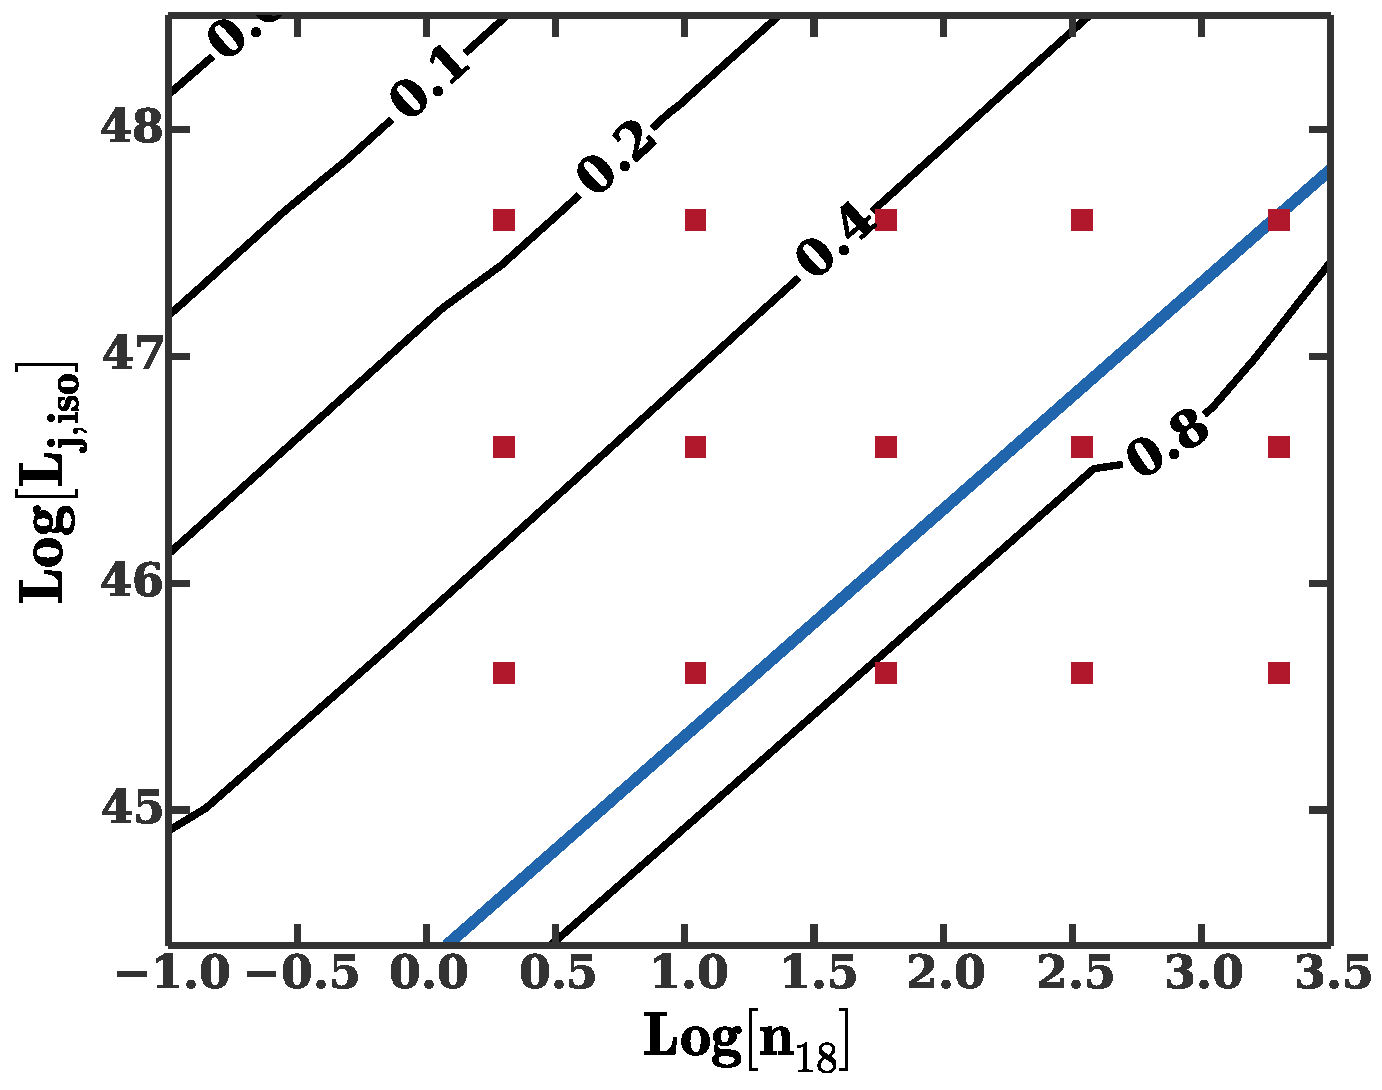
\includegraphics[width=8cm]{diss.pdf}
\caption{\label{fig:diss} Fraction of the slow component
  ($\Gamma_j=2$) kinetic energy dissipated by the reverse shock
  vs. the isotropic jet luminosity ($L_{\rm j,iso}$) and $n_{18}$.}
\end{figure}

\subsection{Jet Models}
\label{sec:numerical}

The jet-CNM interaction is simulated in one and two-dimensions, and
the resulting synchrotron emission is computed using the same
procedure described in \citet{Mimica+2015}. We assume the same angular
Lorentz factor dependence as in previous paper (i.e., $\Gamma = 10$
for the fast inner core and $\Gamma = 2$ for the slow outer sheath),
but we introduce a number of modifications regarding the jet energy
when performing 1D simulations.

\subsection{1D vs. 2D Models}
\label{sec:2D}

The preferred numerical model for Swift J1644+57 \citep[Fig.10
in][]{Mimica+2015} was obtained using 2D simulations (the red line in
that figure). However, the light curve of a 1D version of the same
model \citep[black line in Fig. 10 in][see also section 4.2 of that
paper]{Mimica+2015} matches the 2D light curve only at early times,
when the emission from the inner relativistic jet dominates, while at
late times, when the emission from the slow outer core dominates, the
1D model overestimates the emission from the 2D model. In this work we
found a modification of the 1D model that made its light curves
match the 2D results much more closely.

We first summarize the two-component model as presented in
\citet{Mimica+2015}. The jet has a fast inner core spans an angular
interval $[0, 0.1\ {\rm rad}]$, while the slow outer sheath occupies
$[0.1\ {\rm rad}, 0.5\ {\rm rad}]$. For both components we assume
$E_{\rm ISO} = 4\times 10^{54}$ erg. The crucial thing to notice is
that, keeping $E_{\rm ISO}$ constant, the true jet energy depends only
on the angular interval: $E_{\rm jet} = E_{\rm ISO} (\cos\theta_{\rm
  j,min} - \cos\theta_{\rm j,max})$. The hydrodynamic evolution of the
components is independent of angle in 1D simulations, but the
radiative transfer/light curve calculation is sensitive to the jet
geometry.

Second, we note that, although the sheath is injected in a relatively
narrow angular interval, at late stages of the jet evolution the bow
shock created by its interaction with CNM spans a much larger interval,
i.e. the slow component becomes almost isotropic \citep[bottom two
panels in Fig. 8 in][]{Mimica+2015}. This is the reason for the
discrepancy with the 1D simulation, because there the slow component
angular size is fixed to the initial one. We note that the stage at
which the jet becomes ``isotropic'' depends on the CNM density,
i.e. the denser the CNM, the faster this is expected to happen.

Since the agreement between 1D and 2D models is good for early
times (when the fast component dominates), we modify only the slow
component in 1D models. We assume that is spans $[0.1\ {\rm rad},
\pi/2\ {\rm rad}]$ and lower its $E_{\rm ISO}$ so that the true jet
energy remains unchanged with respect to the original model:
\begin{equation}\label{eq:Eiso}
 E_{\rm ISO, new} = E_{\rm ISO} \left(\frac{\cos(0.1) - \cos(0.5)}{\cos(0.1) - \cos(\pi/2)}\right)\approx 0.12 E_{\rm ISO}\, .
\end{equation}

We assume the same time dependence for the jet luminosity as in
\citet{Mimica+2015},
\begin{equation}\label{eq:lum}
L_{\rm j, ISO}(t) = L_{j,0}\max\left[1, (t/t_0)\right]^{-5/3}
\end{equation}
where $t_0 = 5\times 10^5$ seconds. Integrating equation~\ref{eq:lum}
in time from $0$ to $\infty$ would give $E_{\rm ISO}$. Thus,
$L_{j,0}=0.4\, E_{\rm ISO}/t_0$. 

We show a comparison of this modified 1D approach with the true 2D
result in Figure~\ref{fig:1D2DB}, for $n_{18}=60$ and $n_{18}=2000$
and $E_{\rm ISO}=4 \times 10^{54}$ ergs. For $n_{18}=2000$ the
agreement is excellent, while for $n_{18}=60$ the 1D models still
over-predict still over-predict the flux at times after the peak of
the light curve.

We summarize our fiducial jet model in Table~\ref{tab:jetParams}.

\begin{table}
  \caption{\label{tab:jetParams}Parameters for our jet model}
  \begin{tabular}{ll}
    \hline
    Fast component\\ 
    $\Gamma_j$ & 10 \\
    $[\theta_{\rm min}$, $\theta_{\rm max}]$ & [0, 0.1] radians \\
    $E_{\rm ISO}$ & $4 \times 10^{54}$ ergs \\
    $E$ & $2 \times 10^{52}$ ergs\\
    $L_{\rm j,ISO}$ & $L_{j,0} \max\left[1, (t/t_0)\right]^{-5/3}$  \\
    $t_0$ & $5\times 10^5$ s\\
    $L_{j,0}$ & $3.2 \times 10^{48}$ ergs/s\\
    \hline 
    Slow component\\
    $\Gamma_j$ & 2 \\
    $[\theta_{\rm min}$, $\theta_{\rm max}]$ & [0.1, $\pi/2$] radians \\
    $E_{\rm ISO}$ & $4.7 \times 10^{53}$ ergs \\
    $E$ & $4.7 \times 10^{53}$ ergs\\
    $L_{\rm j, ISO}$ & $L_{j,0} \max\left[1, (t/t_0)\right]^{-5/3}$  \\
    $t_0$ & $5\times 10^5$ s\\
    $L_{j,0}$ & $3.8 \times 10^{47}$ ergs/s\\
    \hline
    Micro-physical parameters\\
    $\epsilon_e$ & 0.1\\
    $\epsilon_b$ & 0.002\\
    $p$ & 2.3\\
  \end{tabular}
\end{table}



\begin{figure*}
\includegraphics[width=16cm]{1D_2D.pdf}
\caption{\label{fig:1D2DB} Comparison of 1D and 2D light curves for
  $n_{18}=60$ (top) and $n_{18}=2000$ (bottom) for frequencies of 1
  GHz (left) and 5 GHz (right) and an observer angle of 0.8 radians
  to the jet axis. We assume an $n\propto r^{-1}$ density profile for
  $n_{18}=2000$, but take $n\propto r^{-1.5}$ for $n_{18}=60$ for
  computational convenience--this model was previously computed in
  \citet{Mimica+2015} and 1D results suggest that the density slope would
  have minimal impact on the results (see $\S$~\ref{sec:profileComp})}.
\end{figure*}

\section{Results}
\label{sec:results}
We have computed on-axis radio light curves across a grid of CNM
densities and jet energies. We use three different values for the
jet energy ($5 \times 10^{51}$, $5 \times 10^{52}$, and $5 \times
10^{53}$ ergs) and five different values for $n_{18}$ (2, 11, 60, 345,
and 2000 cm$^{-3}$). 

We show isocontours of the peak time, $t_p$, and the peak luminosity,
$\nu L_{\nu, p}$, in Fig.~\ref{fig:jetContours} below. We find the
following analytic formula roughly reproduces the behavior of the peak
luminosity across our grid:

\begin{equation}
\nu L_{\nu, p}=2.6 \times 10^{41} \left(\frac{E}{5 \times 10^{53}
    {\rm ergs}}\right)^{0.9}
\left(\frac{\nu}{5 {\rm GHz}}\right)^{1.8} {\rm ergs/s}
\label{eq:peakLum}
\end{equation}

\begin{figure*}
  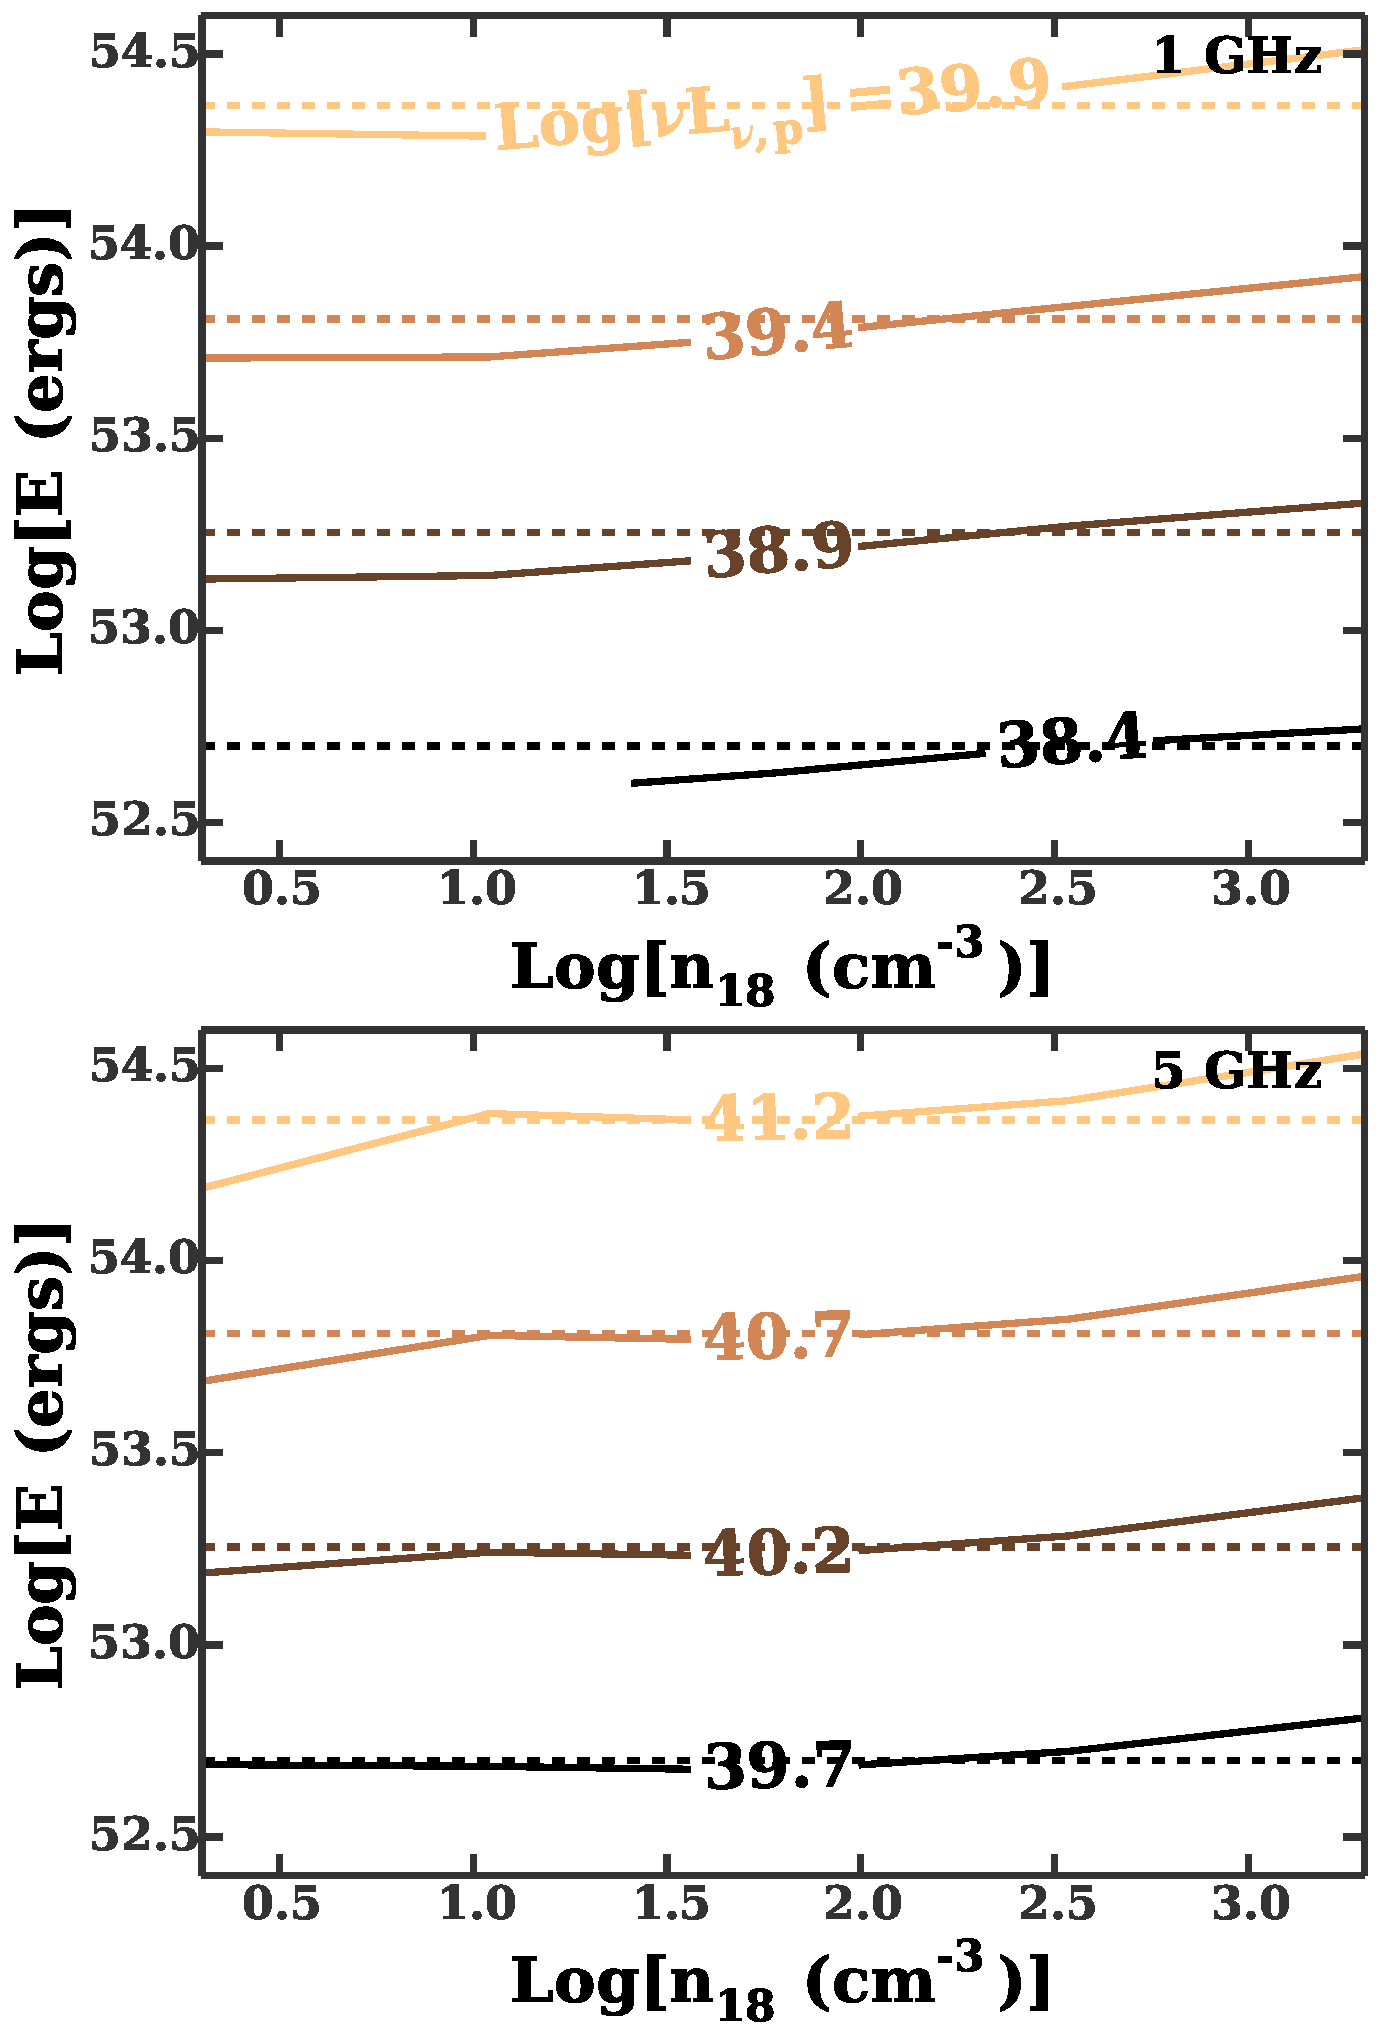
\includegraphics[width=8cm]{lp_contours.pdf}
  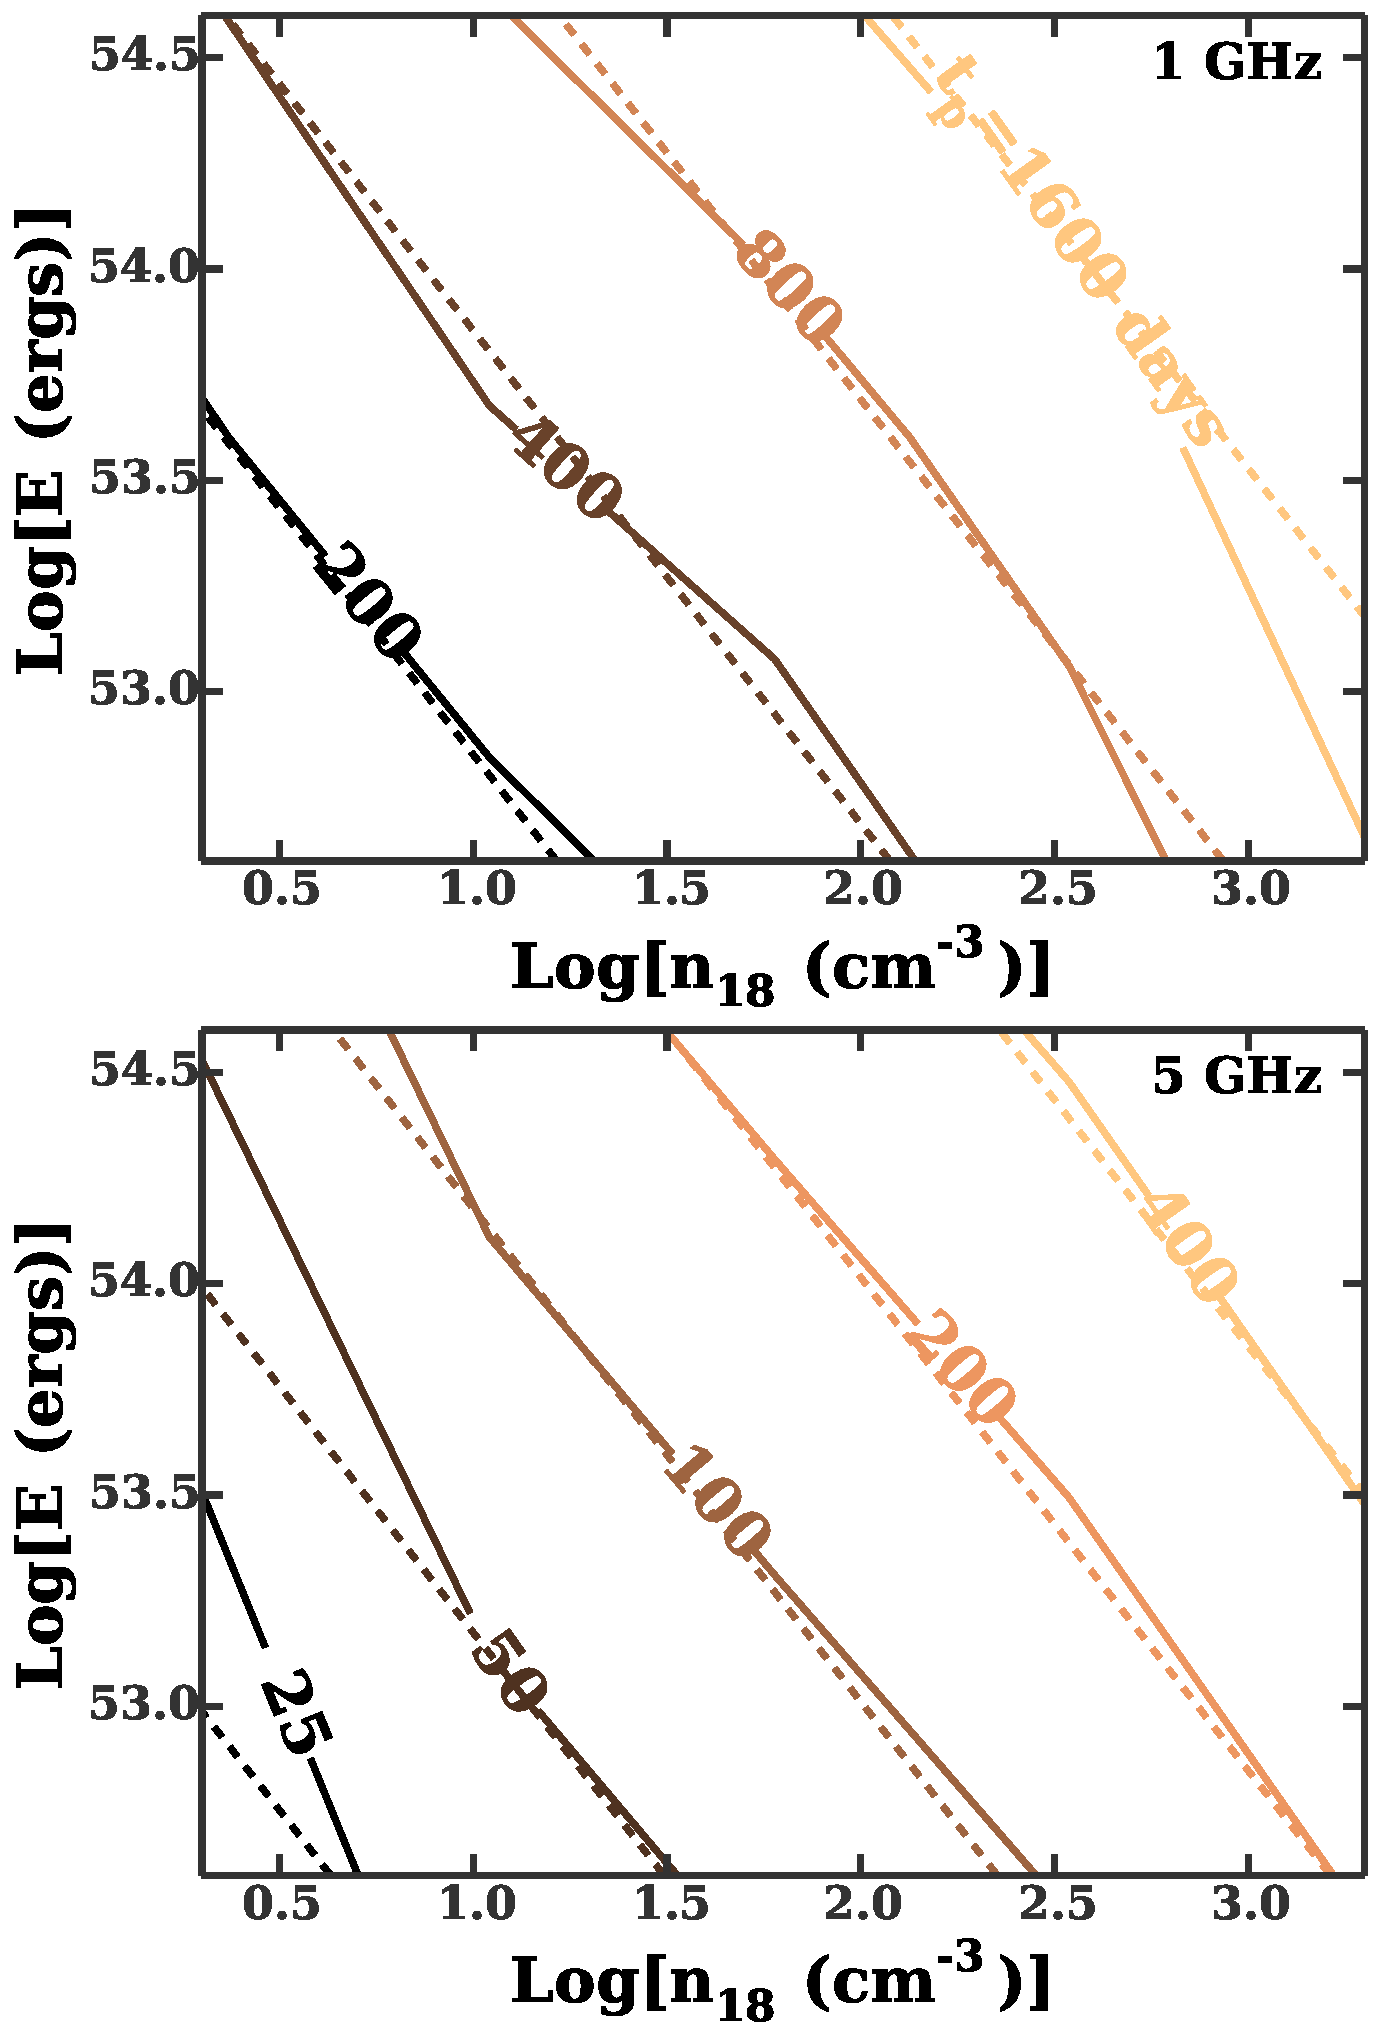
\includegraphics[width=8cm]{tp_contours.pdf}
  \caption{\label{fig:jetContours} Isocontours of peak radio
    luminosity and peak time for a jet of energy $E$ interacting with
    nuclear gas with density profile $n=n_{18}
    \left(r/10^{18}\right)^{-1}$ (\textit{solid lines}). The jet model is described in 
  $\S$~\ref{sec:2D}. We also see analytic fits (see
  equations~\eqref{eq:peakTime} and~\eqref{eq:peakLum}) to the
  numerical results as dashed lines.}
\end{figure*}


Remarkably, we find that the peak luminosity is only weakly dependent
on density across most of the parameter space. In the optically thin
limit the peak luminosity scales as the density $n^{0.5}$. In our case the
jet is initially optically thick and then becomes optically thin at
later times. In fact, the peak of the light curves occurs, when the total
optical depth of the jet is $\sim 1$. {\bf AG need to explain why the
  dependence on density is so weak...}


We also find the following relation fitting formula for the time of
peak, $t_p$, 

\begin{equation}
t_p = 39.5 \left(\frac{E}{5 \times 10^{53} {\rm ergs}}\right)^{0.3} 
\left(\frac{\nu}{5 {\rm GHz}}\right)^{-1} n_{18}^{0.35} {\rm days}
\label{eq:peakTime}
\end{equation}

Note that the peak time occurs later for larger $n_{18}$, as the
transition from optically thick to optically thin occurs at later times.

\subsection{Emission by components}
Our radio light curves include contributions from both the fast
$\Gamma=10$ core and the slow $\Gamma=2$ sheath. In general, the fast
component is more important for earlier times, higher frequencies, and
lower densities. 

We show the relative contributions of the fast and slow components to
the 5 GHz light curve of a $5 \times 10^{53}$ erg jet going through
different gas densities. For $n_{18}=2000$, the slow component
dominates for nearly all times.  For $n_{18}=2$, the fast component
dominates at early times and at the peak of the light curve, while the
slow component dominates after $\sim$1 year.


\begin{figure}
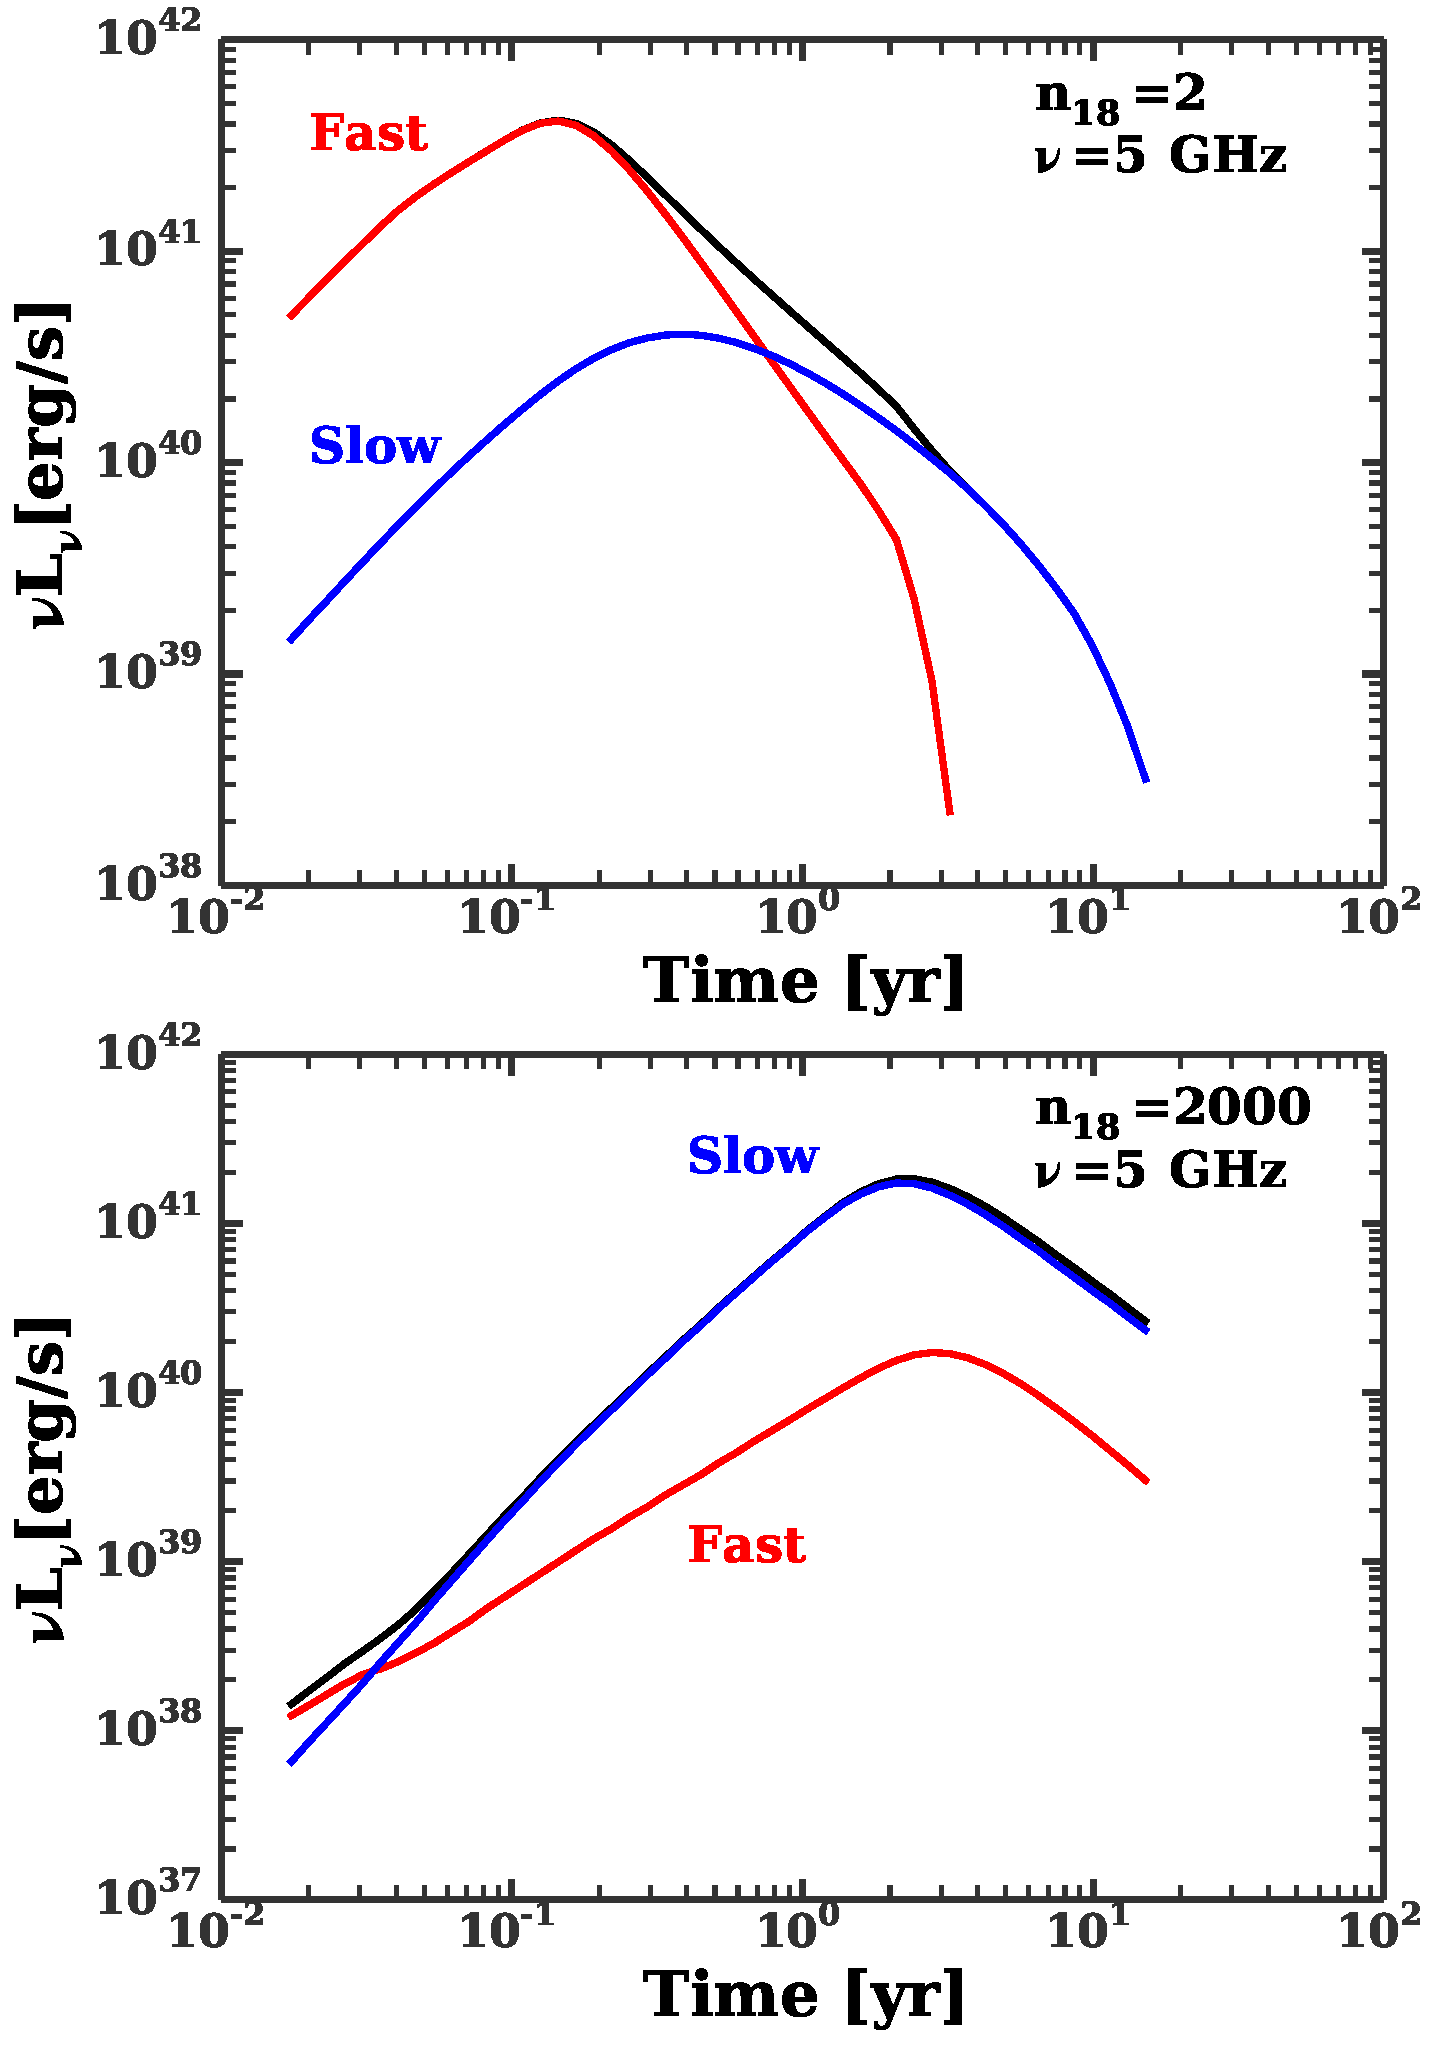
\includegraphics[width=8cm]{components.pdf}
\caption{\label{fig:components} Contributions from the fast
  (\textit{red}) and slow (\textit{blue}) to the 5 GHz light curves
  (\textit{black}) for $n_{18}=2$ (\textit{top}) and $n_{18}=2000$
  (\textit{bottom}).}
\end{figure}

We don't include emission from the reverse
shock. Generally, we expect it would be either self-absorbed or
absorbed by the forward shock. However, emission from the reverse
shock may be important for \textbf{...AG flesh out} 

\subsection{Comparison with radio detections and upper limits.}

In the left panel of Fig.~\ref{fig:lightcurves} we show on-axis light
curves for a $5\times 10^{53}$ erg jet (comparable to Sw1644) and a
few different densities: n$_{18}$: 2, 60, and 2000 cm$^{-3}$ together
with radio upper limits and detections for various TDE candidates in
Fig.~\ref{fig:lightcurves} (these were compiled from various sources
into Table 1 of \citealt{Mimica+2015}).  All of the 5 GHz light curves
fall above the upper limits. However, we were unable to perform a 2D
calculation for $n_{18}=2$.  For $n_{18}=60$, the 2D light curve falls
$\sim$one order of magnitude below the 1D light curve after $\sim$ 10
years. Thus, we caution that the 1D light curves for $n_{18}=2$ likely
overestimate the late time radio luminosity. For this density even a
Sw1644 like jet would fall below existing upper limits. As shown in
the right-hand panel of Fig.~\ref{fig:lightcurves}, for a jet two
orders of magnitude lower in energy, the light curves are either
comparable to or below existing upper limits.

Multiple radio measurements from several months to a few years after a
tidal disruption flare would provide better constraints on the
presence of TDE jets. Non-detections would rule out jets with $\gsim
1\%$ of the energy of Sw1644.



\begin{figure*} 
  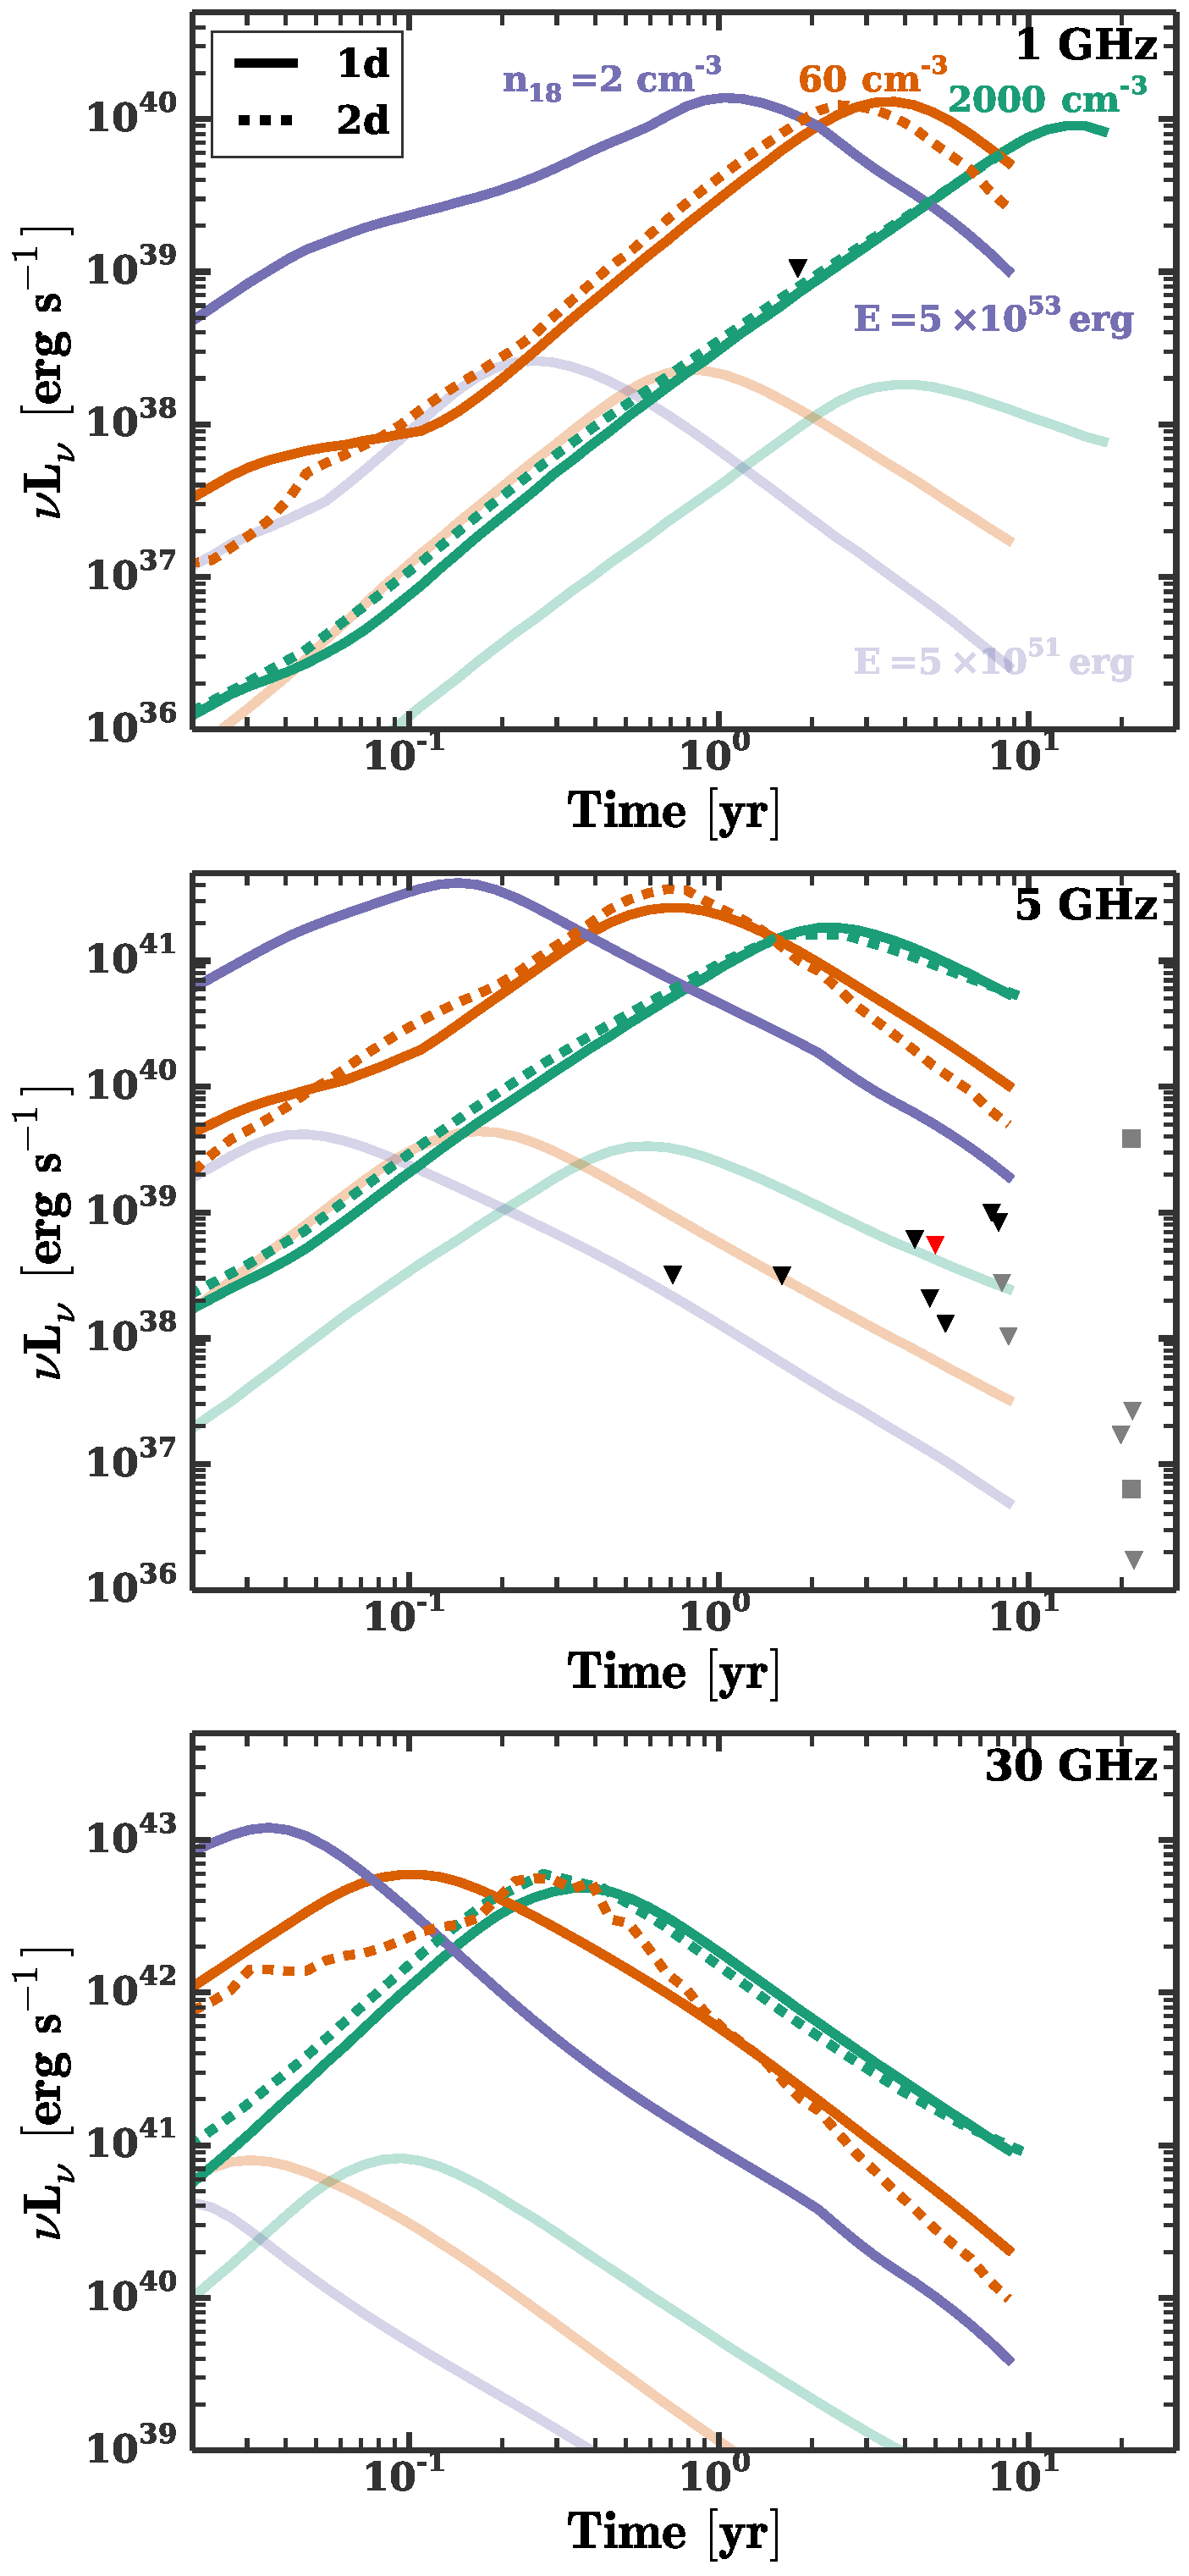
\includegraphics[width=8cm]{lightcurves.pdf}
  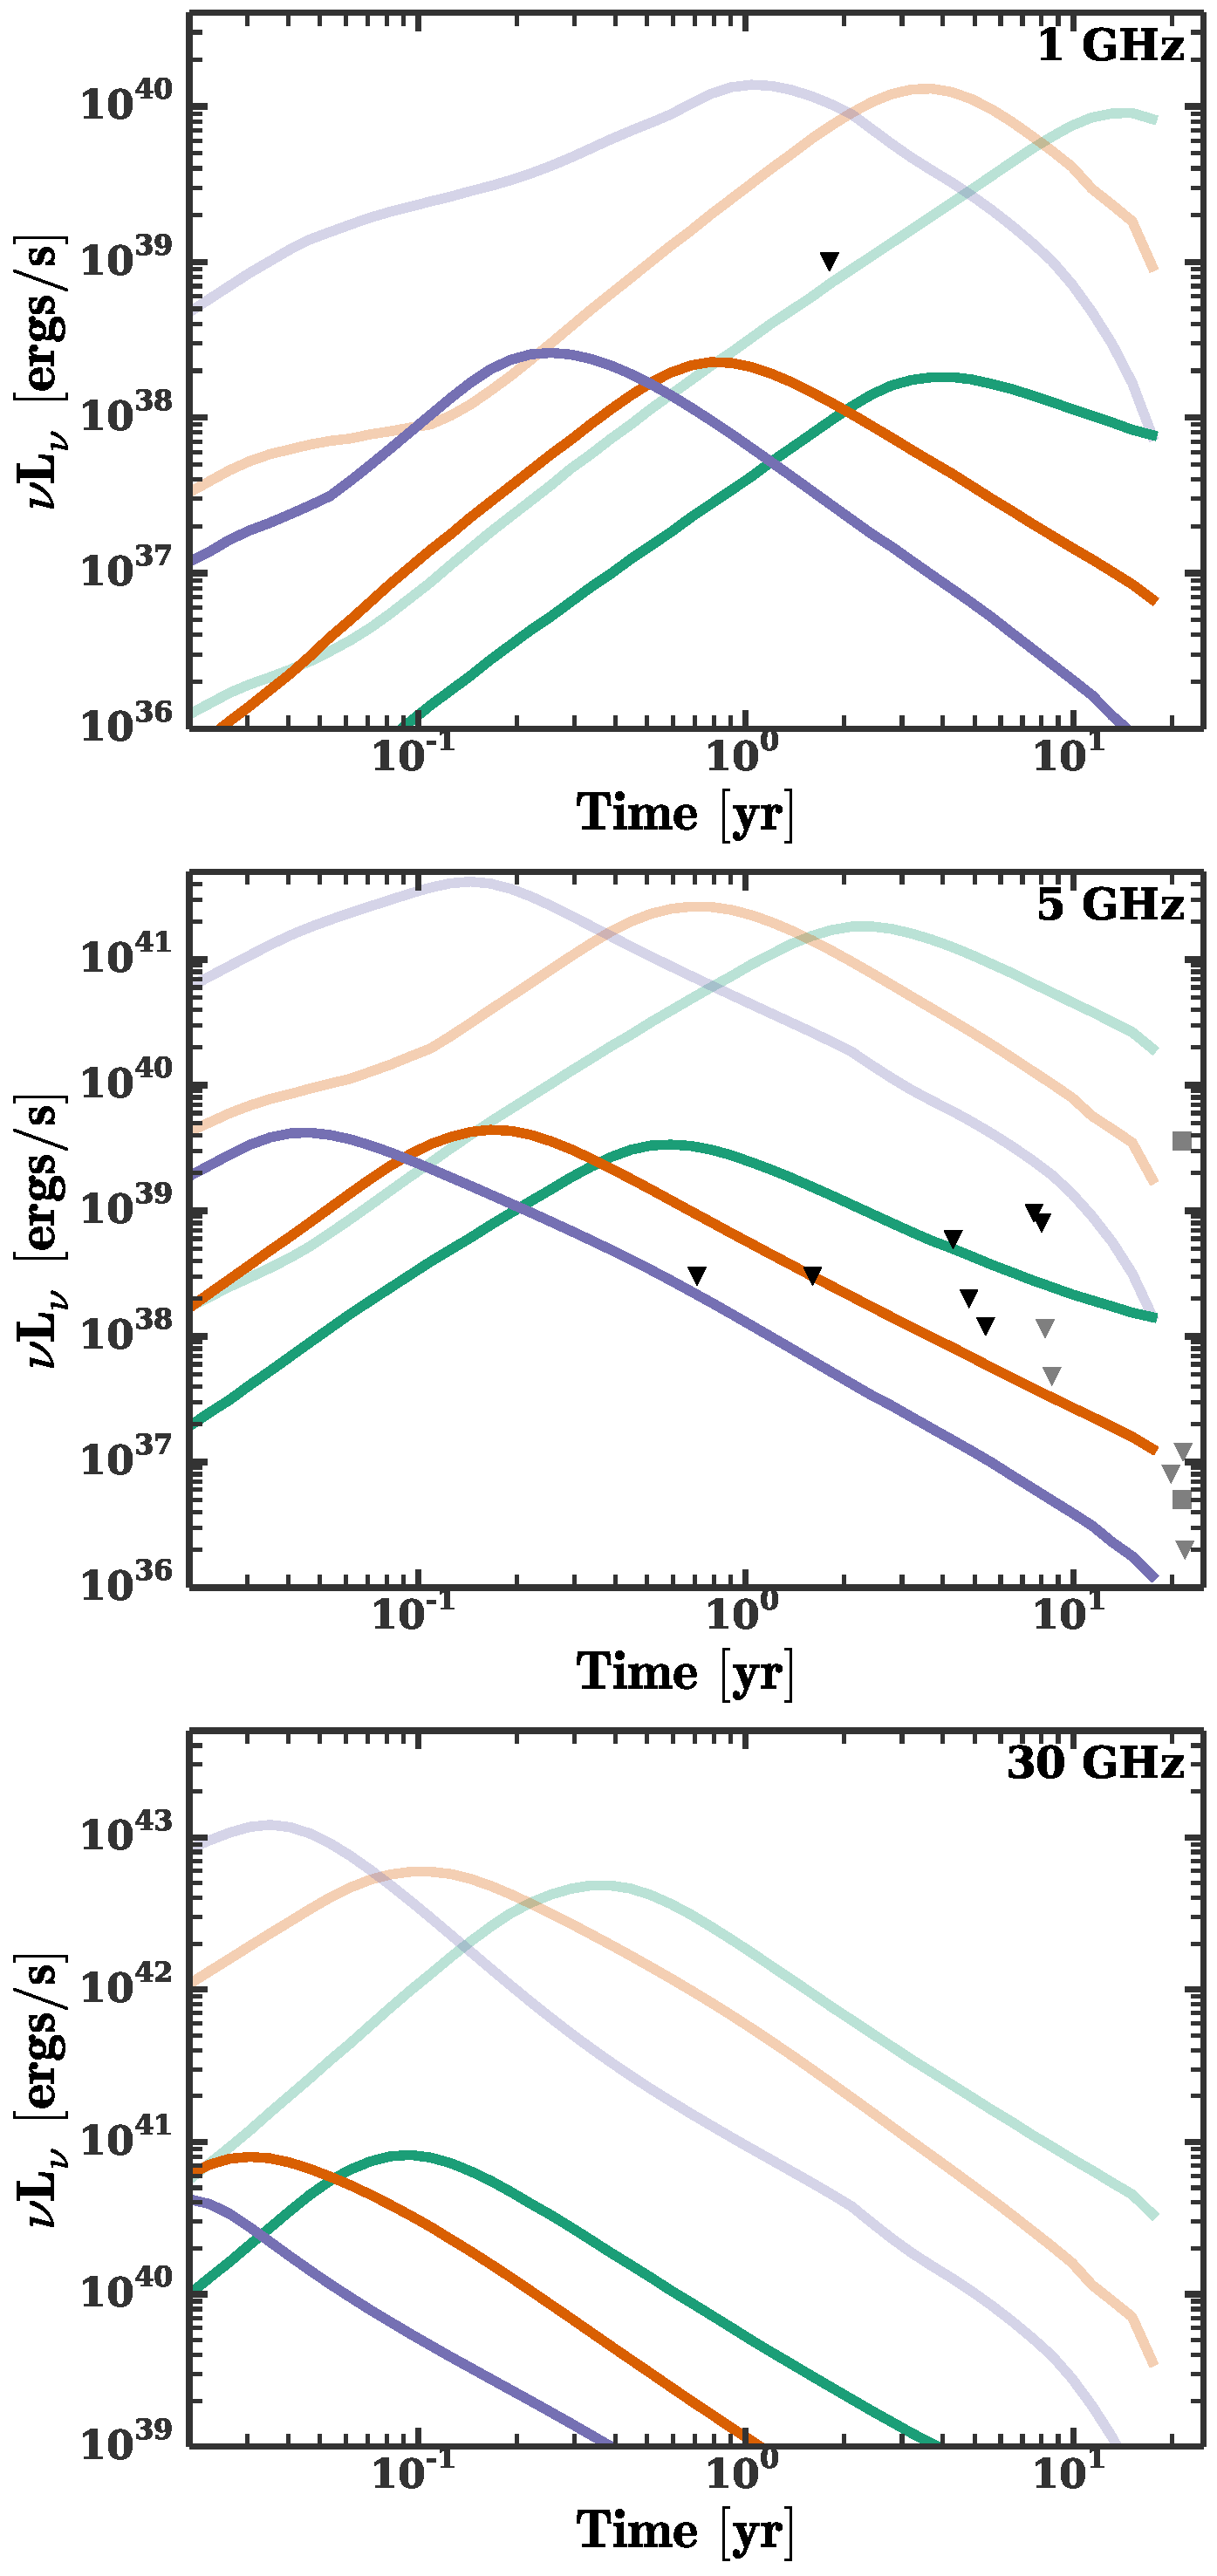
\includegraphics[width=8cm]{lightcurves_en.pdf}
  \caption{\label{fig:lightcurves} \textit{Right-hand panel:} On-axis
    ($\theta_{\rm obs}=0$) radio light curves for our fiducial jet
    model and three different values of n$_{18}$: 2, 60, and
    2000. Solid lines correspond to the light curves from 1D jet
    simulations. When available ($n_{18}=60$ and $n_{18}$=2000), we
    have plotted light curves from the 2D jet simulations as dashed
    lines. Note we use $n\propto r^{-1}$ for $n_{18}=$ 2 and 2000, but
    $r^{-1.5}$ for $n_{18}=60$, as this model had already been
    computed and since the 1D results suggest that the density slope
    will have minimal impact on the results (see
    $\S$~\ref{sec:profileComp}).  Radio upper limits and detections
    are shown as black/gray triangles and squares respectively
    (compiled in Table 1 of \citealt{Mimica+2015}). The single upper
    limit in the top panel corresponds to 1.4 GHz. Gray triangles and
    squares in the middle panel indicate upper limits and detections
    at 3.0 GHz, while black triangles indicate upper limits at 5.0
    GHz. \textit{Left-hand panel} 1D on-axis light curves for a jet
    with a total energy of $5\times 10^{51}$ ergs, together with radio
    upper limits and the light curves for our fiducial case
    (translucent lines).}
\end{figure*}

\subsection{Effects of viewing angle}
We show a comparison off and on-axis light curves in
Fig.~\ref{fig:onOff}.  For $n_{18}=2000$ the light curves differ
little.  For $n_{18}=60$ off-axis luminosity is lower by a factor of a few
before and near the peak. However, for late times
the off- and on-axis light curves are quite similar. This is as
expected, at late times the jet becomes more isotropic, which means
the viewing angle has relatively little effect on the observed light curve.

\begin{figure*}
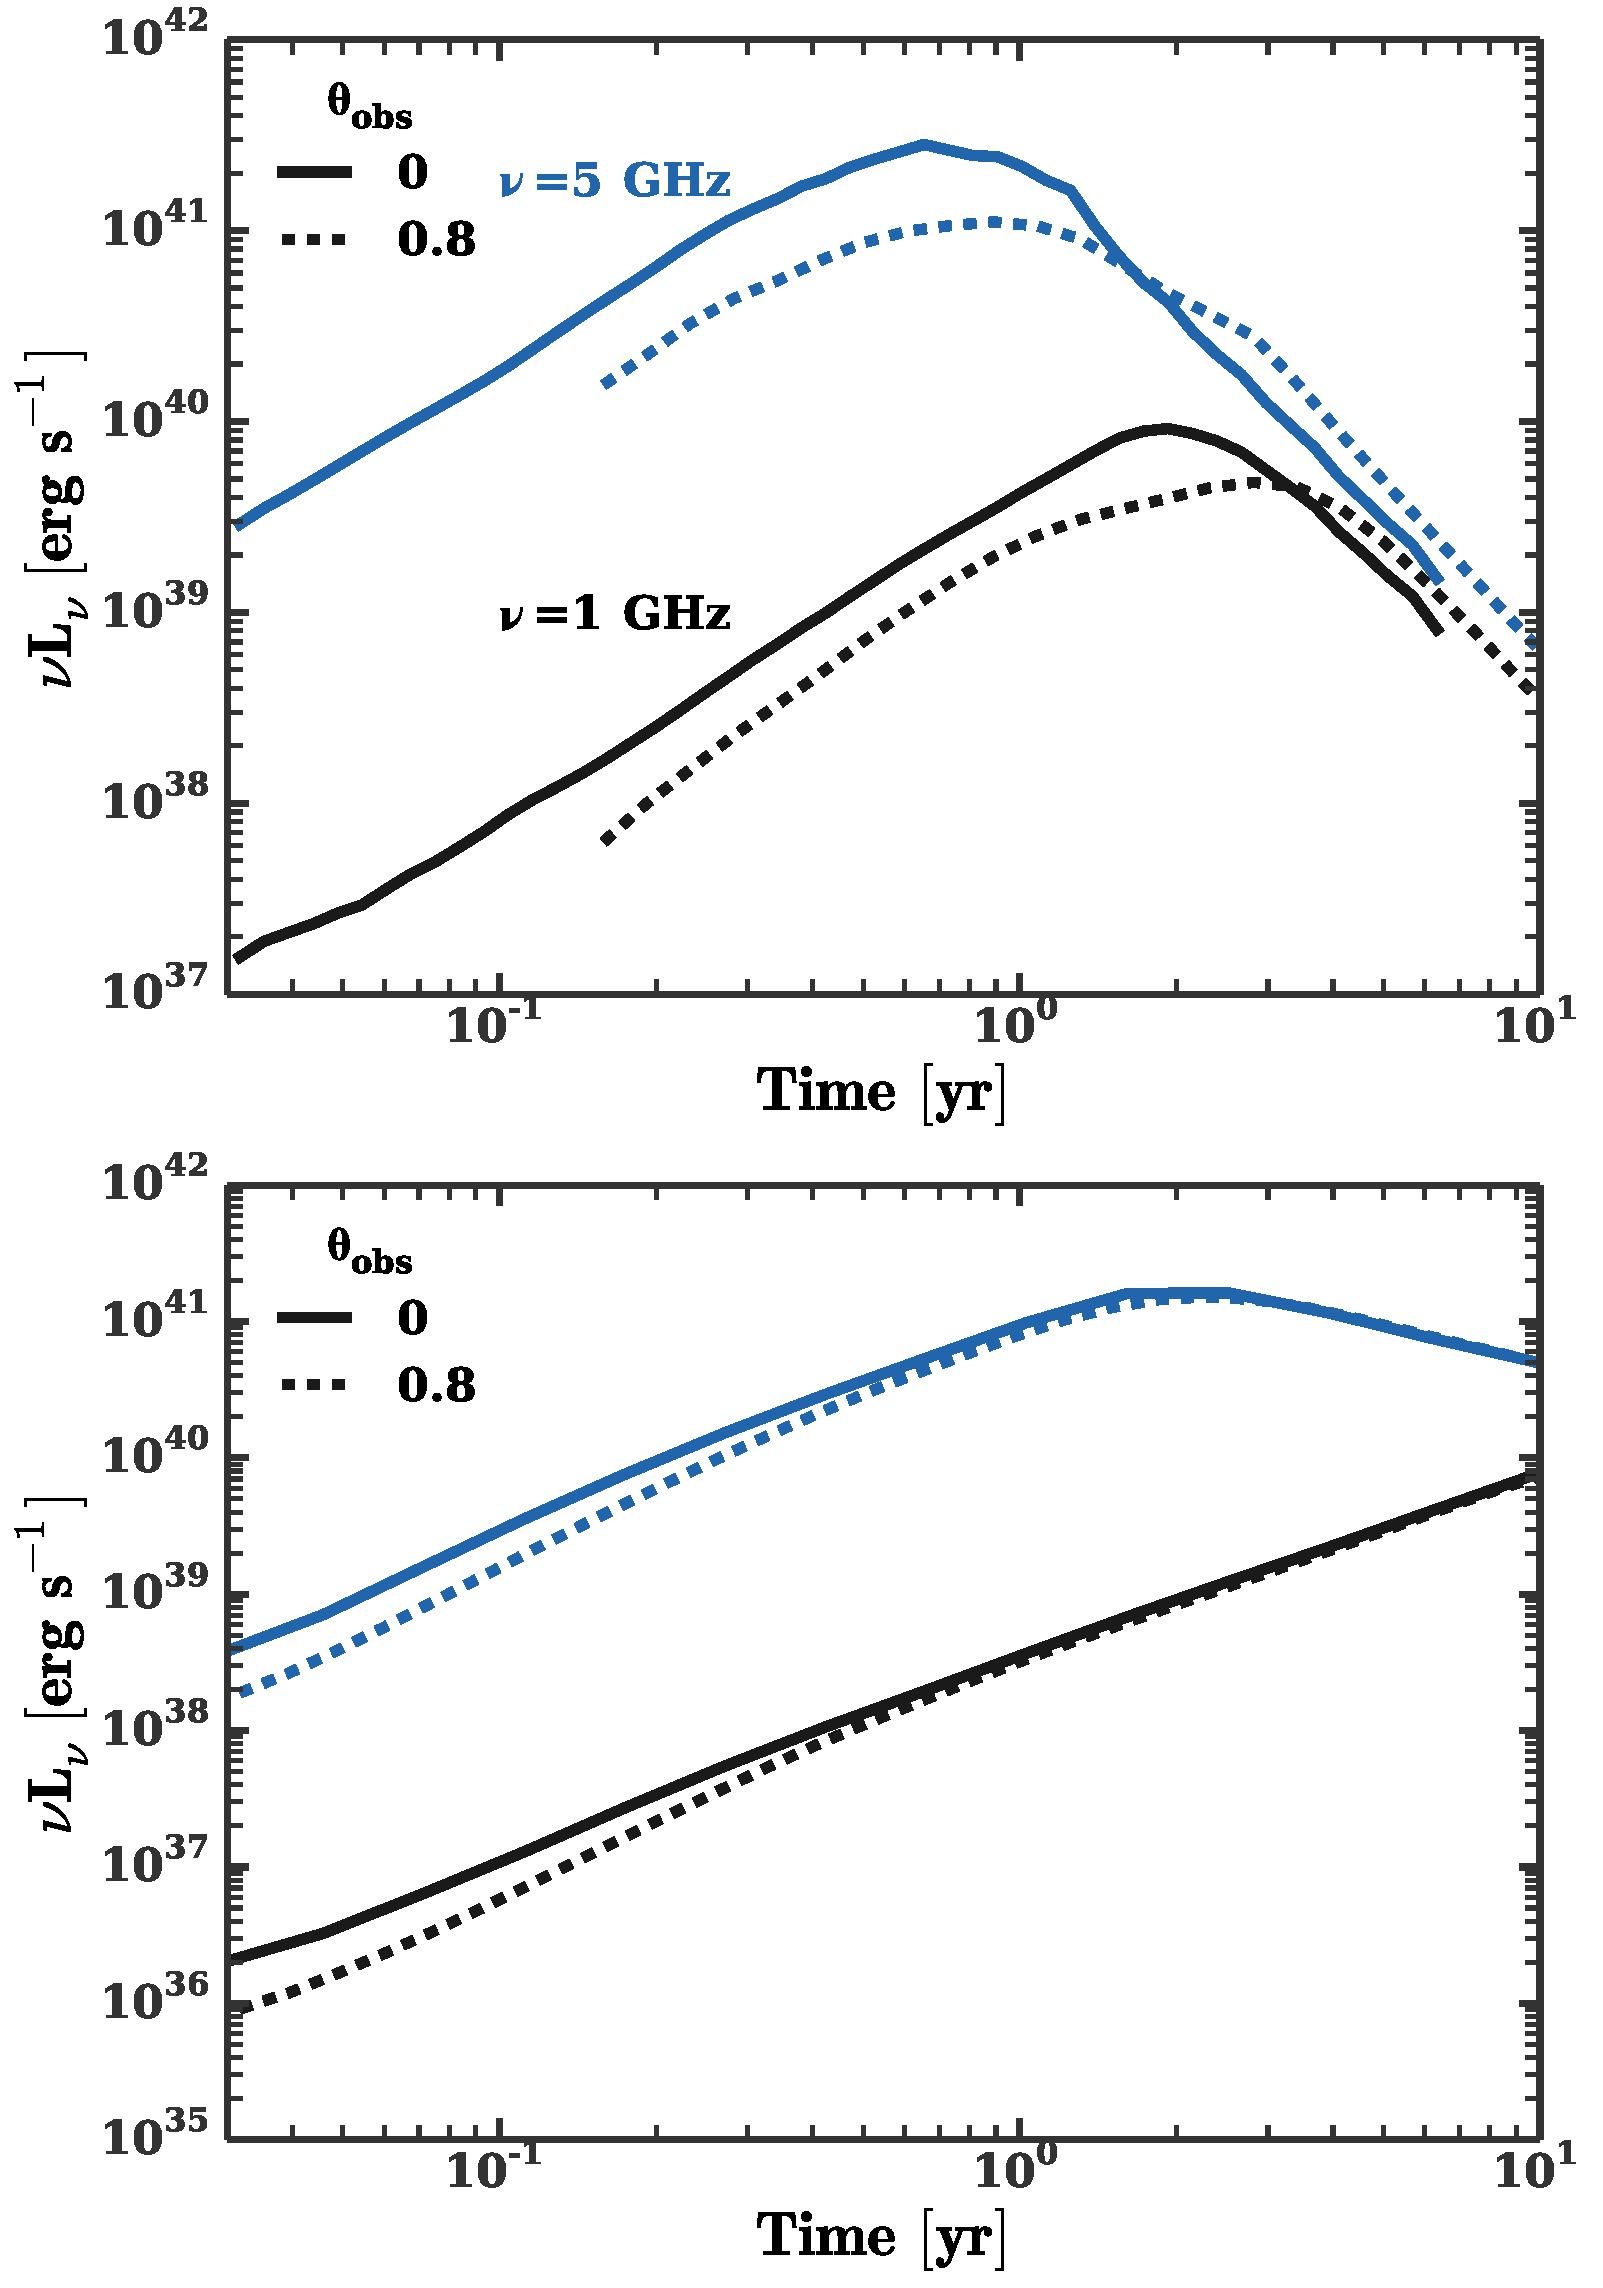
\includegraphics[width=16cm]{on_off.pdf}
\caption{\label{fig:onOff} Comparison of (2D) off- and on-axis
  light curves for $n_{18}=60$ (top) and $n_{18}=2000$ (bottom) for
  frequencies of 1 GHz (left) and 5 GHz (right). The observer line of
  sight is taken to be at $\theta_{\rm obs}=0.8$ with respect to the
  jet axis. We assume an $n\sim r^{-1}$ density profile for
  $n_{18}=2000$, but take $n\sim r^{-1.5}$ for $n_{18}=60$ for
  computational convenience.}
\end{figure*}

% \subsection{Effect of jet energy}
% In the left-hand panel of Figure~\ref{fig:lightcurves} we show radio
% light curves for a jet with energy $E=5\times 10^{51}$ ergs--two
% orders of magnitude smaller than for the high energy jet.  The peak
% luminosities are also $\sim$ two orders of magnitude lower, as the
% peak luminosity is approximately linear in jet energy. 

% For low densities ($n_{18}\sim 60$ cm$^{-3}$) the radio light curves
% for the low energy jet fall below the observed radio upper limits at
% late times. 


\subsection{Effect of gas density profile}
\label{sec:profileComp}
We have also computed the radio light curves for different shapes of
the gas density profile, while holding $n_{18}$ fixed. We compute the
results for $n_{18}=2000$ for both our fiducial $n\propto r^{-1}$ profile and
the core galaxy profile, shown in equation~\eqref{eq:cores}. 
% The
% former would more relevant for a cuspy stellar density profile with
% stellar density $\rho_{\star}\propto r^{-2}$, while the latter would be more
% appropriate for a flatter $\rho_{\star}\propto r^{-1}$ stellar density
% profile. As a steeper stellar density is more favorable for producing
% tidal disruption events, we would expect most events to occur is cusp
% rather than core galaxies.

The on-axis light curves are virtually indistinguishable as shown in
Fig.~\ref{fig:cores}. This result is not surprising as
the core and cusp profiles are quite similar inside of $10^{18}$ cm,
and we expect the jet to have decelerated inside of this radius for
these high densities. 

In Fig.~\ref{fig:profs2} we compare the 1D on-axis light curves for
density two density profiles: $n\propto r^{-1}$ and $n\propto r^{-1.5}$
with $n_{18}=60$. Once again the results are quite similar. Again this
is not surprising as the models have the same density near the Sedov
radius ($\sim 10^{18}$ cm).  


\begin{figure} 
  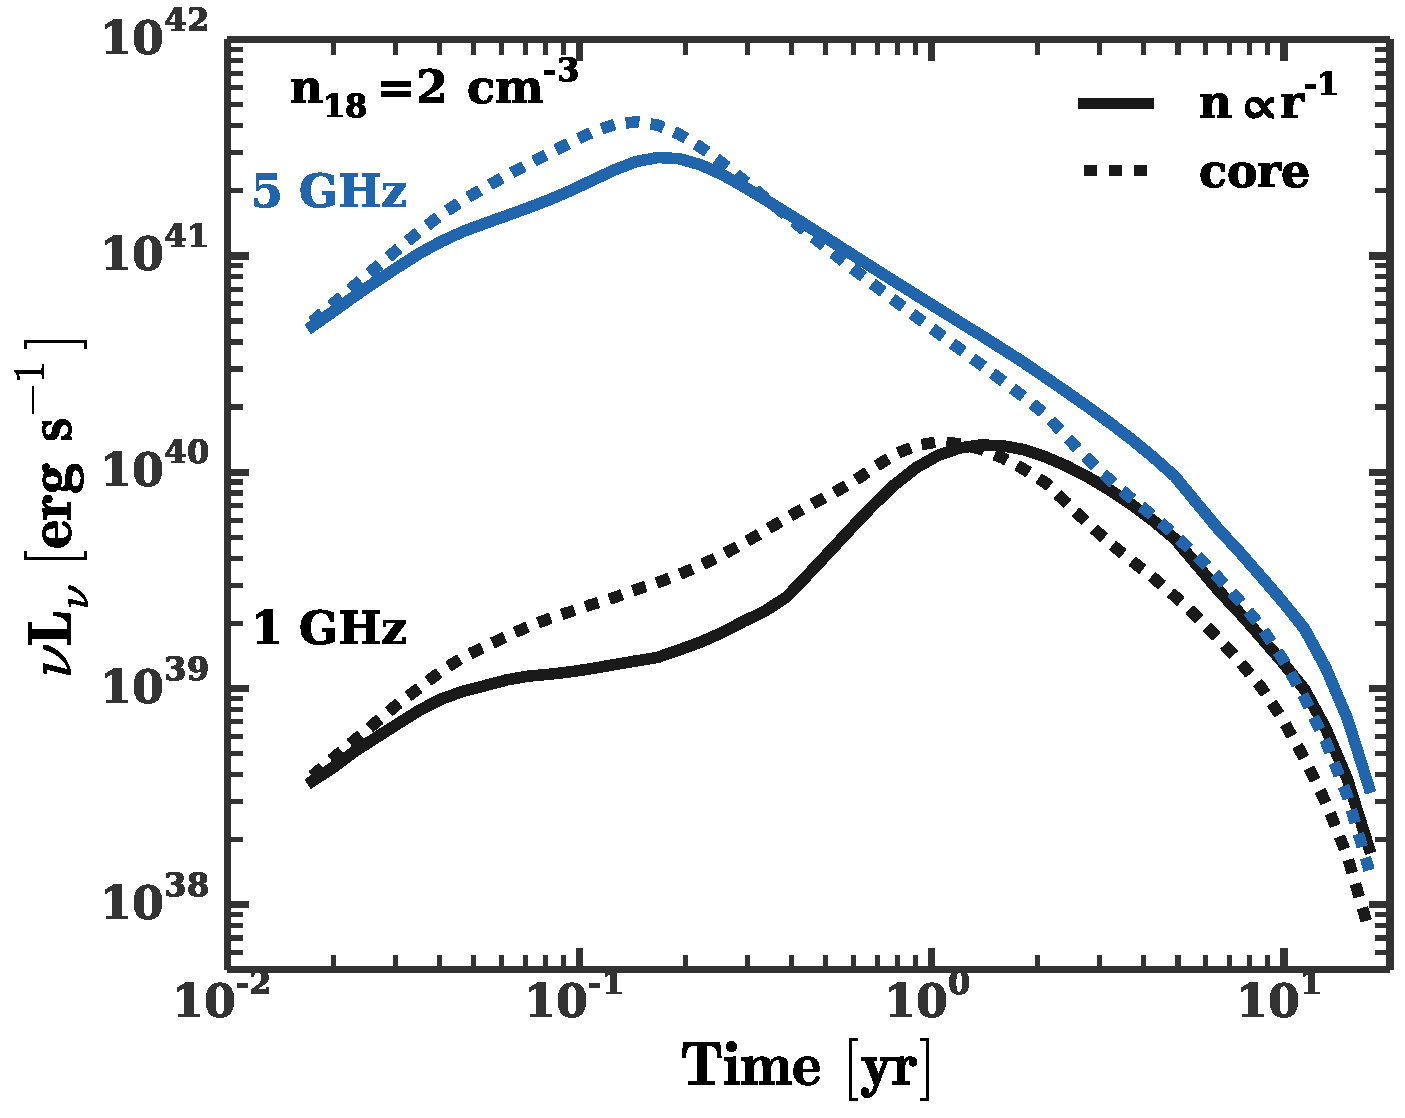
\includegraphics[width=8cm]{fig_cores.pdf}
  \caption{\label{fig:cores} Comparison of (on-axis) light curves for
    $n_{18}=2000$ and two different CNM gas density profiles: $n\sim
    r^{-1}$ and the core galaxy profile from \eqref{eq:cores} with
    $r_s=10^{18}$ cm and $n(r_s)=2000$, so that we can isolate the
    effect of the shape of the density profile.}
\end{figure}


\begin{figure} 
  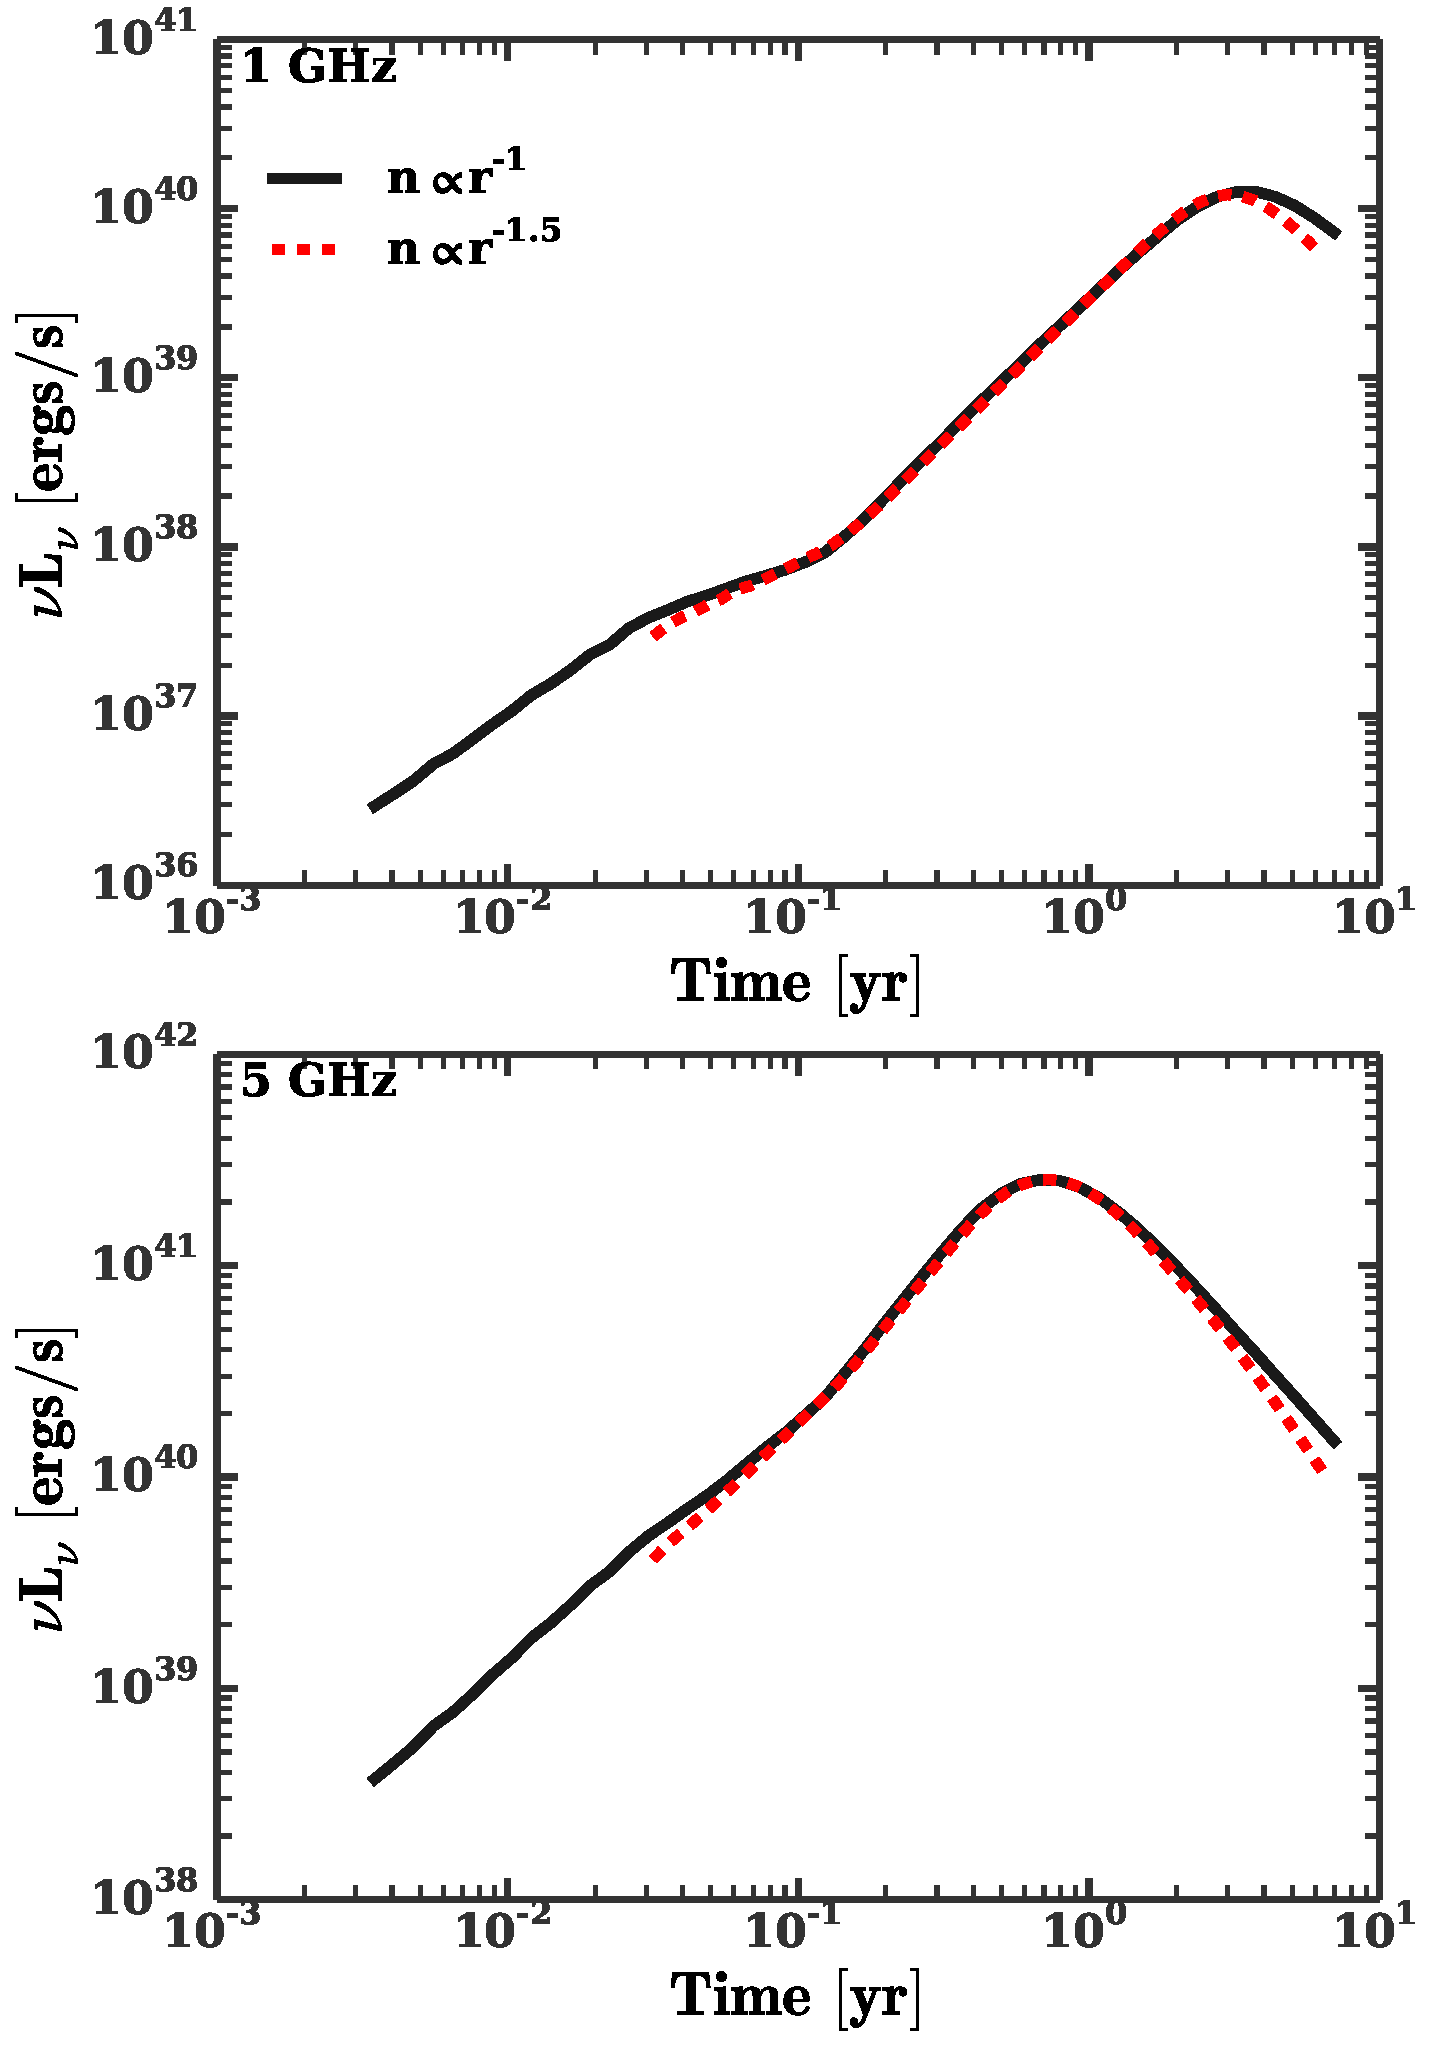
\includegraphics[width=8cm]{profs2.pdf}
  \caption{\label{fig:profs2} Comparison of (on-axis) light curves for
    $n_{18}=60$ and two different CNM gas density profiles: $n\propto
    r^{-1}$ ({\it solid black}) and $n\propto r^{-1.5}$ ({\it dashed
      red}).}
\end{figure}



\section{Summary and Conclusions}
\label{sec:conc}

We calculate radio light curves for tidal disruption event jets
propagating through different circumnuclear (CNM) gas densities. We
simulate the jet propagation using both 1D and 2D hydrodynamic
simulations. We then post-process these to produce radio synchrotron
light curves. To isolate the effects of the density profile we take a
fixed two component jet model from \citet{Mimica+2015}, which produces
a good fit to the observed radio data in Sw1644. We
consider a broad range of gas densities motivated by analytic
estimates of stellar wind mass injection and empirical constraints
based on observed distributions of Eddington ratios. Our conclusions
are summarized as follows.

\begin{enumerate}
\item We estimate the hot phase densities expected from injection of
  stellar wind material for different star formation histories. We
  find that that range of gas densities at 10$^{18}$ cm is $n_{18}
  \sim$ 0.5-1000 cm$^{-3}$.

\item The slope of the gas density profile depends on the slope of the
  stellar density profile. We expect a typical TDE host to have cusp
  like stellar density profile inside of a few pc, with $\rho_\star
  \propto r^{-2}$. This translates into a gas density profile $n
  \propto r^{-1}$. The radio light curve of a TDE jet is most
  sensitive to the density at the deceleration/Sedov radius (where it
  has swept up its mass in CNM gas). The light curve will be
  insensitive to changes in slope for fixed density at the
  deceleration radius.

\item We use the distribution of Eddington ratios (measured by
  \citealt{Kauffmann&Heckman2009} using $L[0III]/\Mbh$) for a sample
  $\sim 10^{7} \Msun$ black holes from SDSS to obtain an empirical
  constraint on the average circumnuclear gas density, including all
  phases of gas. We find that $\sim90\%$ of galaxies in the sample
  have $n_{18}<10^{4} {\rm cm}^{-3}$, although we note that there is
  considerable uncertainty in translating an observed Eddington ratio
  to a circumnuclear gas density. TDE hosts would not fall on this
  high density tail, as TDE searches exclude galaxies with evidence of
  AGN activity {\bf AG: not sure if this is accurate statement (TDE
    survey don't explicitly filter on OIII luminosities). But TDE
    hosts don't appear to have very large OIII luminosities.}.

\item We take a jet model which fits the radio data for the Sw1644
  transient (from \citealt{Mimica+2015}) and run it through a range of
  different density profiles. Motivated by the above results for the
  expected range of gas densities we take the density at $10^{18}$ cm,
  to be $n_{18}=2, 60,$ or 2000 cm$^{-3}$. We find bright radio
  emission at a few GHz across this entire range of densities, with
  the peak luminosity only weakly dependent on the chosen value of
  $n_{18}$.  For smaller densities the light curves peak earlier in
  time. Based on existing radio upper limits for tidal disruption
  event candidates, we show Swift 1644-like jet are absent in most TDEs
  as long as the density at $10^{18}$, $n_{18} \gsim  60$
  cm$^{-3}$. Prompt follow-up in the radio could provide tighter
  constraints on the existence of TDE jets.  
\end{enumerate}

\appendix
\section{Core Profile}
\label{app:core}
In $\S\ref{sec:profileComp}$ we compare the results of radio
light curves from jets propagating in core and cusp like gas density
profiles. See Fig.~\ref{fig:profiles} for a comparison of core and
cusp-like profiles. 

We use the following analytic expression to approximate the core
galaxy profile

\begin{align}
\begin{cases}
n=n(r_s) k(x) & 0.4 \leq x\leq 2.0\\
n = 2.0 n(r_s) (x/0.4)^{-0.95} & x < 0.4\\
n = 0.75 n(r_s) (x/2.0)^{-0.26} & x>2.\\
\end{cases}
\label{eq:cores}
\end{align}

Where, 

\begin{align}
  &x=r/r_s\\\nonumber
  &k(x)=\frac{45}{19} \frac{1}{x^{3/2}} \frac{1-x^{1.9}}{9-19
      x\frac{x^{0.9}-1}{x^{1.9}-1}}
\end{align}

To isolate the effects of the shape of the density profile, consider a
core density profile with $r_s=10^{18}$ cm, and $n_{18}=2000$: the
same as our high density cusp model.

\clearpage



\clearpage
  \footnotesize{
    \bibliographystyle{mnras}
    \bibliography{master}
  }

\end{document}
